%===============================================================================
% LaTeX sjabloon voor de bachelorproef toegepaste informatica aan HOGENT
% Meer info op https://github.com/HoGentTIN/bachproef-latex-sjabloon
%===============================================================================

\documentclass{bachproef-tin}

\usepackage{hogent-thesis-titlepage} % Titelpagina conform aan HOGENT huisstijl
\usepackage{float}

%%---------- Documenteigenschappen ---------------------------------------------
% TODO: Vul dit aan met je eigen info:

% De titel van het rapport/bachelorproef
\title{Kwalitatief onderzoek naar integratiemogelijkheden tussen het Microsoft Bot Framework en Microsoft Dynamics 365 for Finance and Operations}

% Je eigen naam
\author{Adil Zarkan}

% De naam van je promotor (lector van de opleiding)
\promotor{Koen Mertens}

% De naam van je co-promotor. Als je promotor ook je opdrachtgever is en je
% dus ook inhoudelijk begeleidt (en enkel dan!), mag je dit leeg laten.
\copromotor{Andy Marijs}

% Indien je bachelorproef in opdracht van/in samenwerking met een bedrijf of
% externe organisatie geschreven is, geef je hier de naam. Zoniet laat je dit
% zoals het is.
\instelling{delaware}

% Academiejaar
\academiejaar{2018-2019}

% Examenperiode
%  - 1e semester = 1e examenperiode => 1
%  - 2e semester = 2e examenperiode => 2
%  - tweede zit  = 3e examenperiode => 3
\examenperiode{2}

%===============================================================================
% Inhoud document
%===============================================================================

\begin{document}
    
    %---------- Taalselectie -------------------------------------------------------
    % Als je je bachelorproef in het Engels schrijft, haal dan onderstaande regel
    % uit commentaar. Let op: de tekst op de voorkaft blijft in het Nederlands, en
    % dat is ook de bedoeling!
    
    %\selectlanguage{english}
    
    %---------- Titelblad ----------------------------------------------------------
    \inserttitlepage
    
    %---------- Samenvatting, voorwoord --------------------------------------------
    \usechapterimagefalse
    %%=============================================================================
%% Voorwoord
%%=============================================================================

\chapter*{\IfLanguageName{dutch}{Woord vooraf}{Preface}}
\label{ch:voorwoord}

%% TODO:
%% Het voorwoord is het enige deel van de bachelorproef waar je vanuit je
%% eigen standpunt (``ik-vorm'') mag schrijven. Je kan hier bv. motiveren
%% waarom jij het onderwerp wil bespreken.
%% Vergeet ook niet te bedanken wie je geholpen/gesteund/... heeft

Met deze bachelorproef wens ik mijn opleiding toegepaste informatica aan de Hogeschool van Gent af te sluiten. De opleiding was zeer leerrijk, en heeft me erg goed klaargestoomd voor de volgende stap in mijn professionele carrière als IT'er, waarvoor dank. Uiteraard wordt een werk van deze omvang nooit alleen geschreven, en wil ik graag van deze kans gebruik maken om enkele mensen te bedanken die me dit hebben helpen realiseren. 

Allereerst wens ik mijn promotor Koen Mertens te bedanken voor de begeleiding, en zijn snelle antwoorden wanneer ik vragen had. Dankzij een eerder moeilijk meetbare onderzoeksvraag verliep vooral de opzet van dit onderzoek stroef. Echter kon meneer Mertens op tijd bijsturen, waarvoor dank.

 Verder ben ik ook het bedrijf delaware, met in het bijzonder mijn co-promotor Andy Marijs en begeleider Ward Lanssens erg dankbaar voor de opportuniteit. Vooral Ward, die me bij zeer veel technische vraagstukken heeft bijgestaan was cruciaal voor het goede verloop van dit onderzoek. 

Mijn voorkennis van zowel het MS Bot Framework als MS Dynamics 365FO was nihil bij het opstarten van deze scriptie, maar dankzij de stevige begeleiding doorheen het hele proces heb ik het tot een goed einde kunnen brengen. Dit deels dankzij leergierigheid van mijn zijde, maar ook dankzij de stevige expertise die men bij delaware door de jaren heen heeft opgebouwd. 

Dankzij deze scriptie heb ik een inzicht verkregen in het Bot Framework enerzijds, maar vooral in Microsoft Dynamics 365FO. Aangezien ik in deze branche ga werken, is de kennis die ik doorheen dit project heb opgebouwd erg nuttig voor het verdere verloop van mijn professionele carrière als business analist binnen het Microsoft Dynamics 365FO Development team binnen delaware. 


    %%=============================================================================
%% Samenvatting
%%=============================================================================

% TODO: De "abstract" of samenvatting is een kernachtige (~ 1 blz. voor een
% thesis) synthese van het document.
%
% Deze aspecten moeten zeker aan bod komen:
% - Context: waarom is dit werk belangrijk?
% - Nood: waarom moest dit onderzocht worden?
% - Taak: wat heb je precies gedaan?
% - Object: wat staat in dit document geschreven?
% - Resultaat: wat was het resultaat?
% - Conclusie: wat is/zijn de belangrijkste conclusie(s)?
% - Perspectief: blijven er nog vragen open die in de toekomst nog kunnen
%    onderzocht worden? Wat is een mogelijk vervolg voor jouw onderzoek?
%
% LET OP! Een samenvatting is GEEN voorwoord!

%%---------- Nederlandse samenvatting -----------------------------------------
%
% TODO: Als je je bachelorproef in het Engels schrijft, moet je eerst een
% Nederlandse samenvatting invoegen. Haal daarvoor onderstaande code uit
% commentaar.
% Wie zijn bachelorproef in het Nederlands schrijft, kan dit negeren, de inhoud
% wordt niet in het document ingevoegd.

\IfLanguageName{english}{%
\selectlanguage{dutch}
\chapter*{Samenvatting}
\lipsum[1-4]
\selectlanguage{english}
}{}

%%---------- Samenvatting -----------------------------------------------------
% De samenvatting in de hoofdtaal van het document

\chapter*{\IfLanguageName{dutch}{Samenvatting}{Abstract}}

\lipsum[1-4]

    
    %---------- Inhoudstafel -------------------------------------------------------
    \pagestyle{empty} % Geen hoofding
    \tableofcontents  % Voeg de inhoudstafel toe
    \cleardoublepage  % Zorg dat volgende hoofstuk op een oneven pagina begint
    \pagestyle{fancy} % Zet hoofding opnieuw aan
    
    %---------- Lijst figuren, afkortingen, ... ------------------------------------
    
    % Indien gewenst kan je hier een lijst van figuren/tabellen opgeven. Geef in
    % dat geval je figuren/tabellen altijd een korte beschrijving:
    %
    %  \caption[korte beschrijving]{uitgebreide beschrijving}
    %
    % De korte beschrijving wordt gebruikt voor deze lijst, de uitgebreide staat bij
    % de figuur of tabel zelf.
    


    \graphicspath{ {img/} }

    
    \listoffigures
    
    \listoftables
    
    % Als je een lijst van afkortingen of termen wil toevoegen, dan hoort die
    % hier thuis. Gebruik bijvoorbeeld de ``glossaries'' package.
    % https://www.overleaf.com/learn/latex/Glossaries
    
    %---------- Kern ---------------------------------------------------------------
    
    % De eerste hoofdstukken van een bachelorproef zijn meestal een inleiding op
    % het onderwerp, literatuurstudie en verantwoording methodologie.
    % Aarzel niet om een meer beschrijvende titel aan deze hoofstukken te geven of
    % om bijvoorbeeld de inleiding en/of stand van zaken over meerdere hoofdstukken
    % te verspreiden!
    %%=============================================================================
%% Begrippenlijst
%%=============================================================================
\chapter{Begrippenlijst}
\label{ch:begrippenlijst}

\section{Gebruikte afkortingen}
\begin{tabular}{|c|c|}
    \hline 
    D365FO &  Microsoft Dynamics 365 for Finance and Operations \\
    \hline 
    MBS & Microsoft Business Solutions \\
    \hline
    CRM & Customer Relationship Management  \\
    \hline
    CEO & Chief Executive Officer \\
    \hline
    AI & Artificiële Intelligentie \\
    \hline
    NLP & Natural Language Processing \\
    \hline
    ERP & Enterprise Resource Planning \\
    \hline
    POC & Proof of concept \\
    \hline 
\end{tabular} 

\subsection{Begrippenlijst}
\subsubsection{User stories}
Korte, simpele beschrijvingen van nieuwe functionele requirements vanuit het perspectief van de gebruiker. (\textcite{Cohn2004})

\subsubsection{Enterprise Resource Planning}
Geïntegreerde informatiesystemen, gebouwd op een gecentraliseerde database die op eenzelfde computer platform draait als de diverse resources van het bedrijf, en op die manier de flow van informatie (over deze resources) tussen alle business functies van het bedrijf faciliteert. (\textcite{Hill2011})

\subsubsection{Stateless, states}

\subsubsection{Serverless}





    %%=============================================================================
%% Inleiding
%%=============================================================================

\chapter{\IfLanguageName{dutch}{Inleiding}{Introduction}}
\label{ch:inleiding}

%De inleiding moet de lezer net genoeg informatie verschaffen om het onderwerp te begrijpen en in te zien waarom de onderzoeksvraag de moeite waard is om te onderzoeken. In de inleiding ga je literatuurverwijzingen beperken, zodat de tekst vlot leesbaar blijft. Je kan de inleiding verder onderverdelen in secties als dit de tekst verduidelijkt. Zaken die aan bod kunnen komen in de inleiding~\autocite{Pollefliet2011}:

%\begin{itemize}
%  \item context, achtergrond
% \item afbakenen van het onderwerp geen optimalisatie bespreken
% \item verantwoording van het onderwerp, methodologie
%\item probleemstelling
%\item onderzoeksdoelstelling
%\item onderzoeksvraag
%\end{itemize}

\section{\IfLanguageName{dutch}{Probleemstelling}{Problem Statement}}
\label{sec:probleemstelling}

\subsubsection{Context en probleemstelling}
Wanneer men naar hedendaagse bedrijfsprocessen, en hun geautomatiseerde systemen kijkt, merkt men vaak éen of meerdere processen op die zéér moeilijk te optimaliseren zijn. Een schoolvoorbeeld hiervan, volgens Andy Marijs van delaware althans, is data-input. Binnen de Microsoft Dynamics afdeling merkt men op dat er een zich een trend voordoet van processen die mits het nodige maatwerk prima optimaliseerbaar zijn, behalve de data-input. Laat dit nu net in veel gevallen het vertrekpunt zijn van courante user stories, wat dus maakt dat deze inefficiëntie vaak aan bod komt. \textcite{TimeXtender2019} stelt manuele data input bovendien zelfs gelijk aan 'errors' en verlies van tijd.

\subsubsection{Scope van het onderzoek}
Concreet werd de Job card device-module binnen Microsoft Dynamics 365 FO door delaware gekozen als te optimaliseren module.\\
Beschrijving module:\\
In de Job Card Device module kunnen medewerkers op de productievloer inloggen met hun badgeID. Nadat ze ingelogd zijn gebruiken ze deze module voor het afmelden van productieorders. Dit wil zeggen, wanneer een goed geproduceerd moet worden (productieorder) kunnen ze via bovenstaande module aanduidden dat ze dat goed gaan beginnen produceren, en wordt er automatisch backflushing gedaan wat gaat registreren hoeveel grondstoffen er mogen geschrapt worden uit de voorraad van het bedrijf. 

Deze module bevat k een aantal operaties, die op vlak van data-input relatief eenvoudig zijn. Echter is het inputten hiervan nog niet maximaal geoptimaliseerd. Het onderzoeken van de specifieke inefficiënties binnen het data input proces reikt buiten de scope van dit onderzoek en zal daarom niet aan bod komen. Ook zal er geen vergelijkende studie worden gemaakt tussen verschillende chatbots en hun mogelijkheden, omdat de opdrachtgever (delaware) gekozen heeft voor het Microsoft Bot Framework. 

\subsubsection{Onderzoeksvraag}
De onderzoeksvraag is daarom om te onderzoeken of (a) het MS Bot Framework complexe/dynamische business processen binnen MS Dynamics 365FO kan
automatiseren. En (b) of de implementatie hiervan nuttig is. 

De keuze voor het Microsoft Bot Framework was een voorwaarde van de opdrachtgever, omdat zij, als Gold Certified Microsoft Partner (\textcite{Delaware2009}), sterke expertise willen ontwikkelen in zaken buiten D365FO binnen het Microsoft ecosysteem. 


Ook biedt het framework out of the box een aantal zaken aan, zoals Language Interpreting, etc. die het technische aspect van de Chatbot voor hun rekening nemen, daar dit uit de scope reikt van de Dynamics afdeling. Ook het feit dat dit framework via Azure werkt, is een groot pluspunt aangezien de authenticatie van Dynamics 365FO via Azure Active Directory dient te verlopen. Uiteraard zijn er andere opties om de chatbot te implementeren, voorbeelden hier van zijn: Dialogflow, Amazon Lex, BotKit, enz.  


stakeholders:
\begin{itemize}
    \item delaware
    \item Microsoft 
    \item Klanten en partners buiten delaware in het D365FO ecosysteem \item Microsoft Bot Framework
    \item MS Dynamics 365 for Finance and Operations
\end{itemize}

\section{\IfLanguageName{dutch}{Onderzoeksvraag}{Research question}}
\label{sec:onderzoeksvraag}
Zorgt het optimaliseren van bepaalde data-input processen binnen Microsoft Dynamics 365 for Finance and Operations door middel van een chatbot geïmplementeerd in het Microsoft Bot Framework voor verhoogde efficiëntie, en is het framework hier klaar voor? 

%Wees zo concreet mogelijk bij het formuleren van je onderzoeksvraag. Een onderzoeksvraag is trouwens iets waar nog niemand op dit moment een antwoord heeft (voor zover je kan nagaan). Het opzoeken van bestaande informatie (bv. ``welke tools bestaan er voor deze toepassing?'') is dus geen onderzoeksvraag. Je kan de onderzoeksvraag verder specifiëren in deelvragen. Bv.~als je onderzoek gaat over performantiemetingen, dan 

Het is belangrijk om het onderzoek in 2 delen op te splitsen. Enerzijds zal er een POC gemaakt worden om te testen of het haalbaar is om de Job card device module deels te vervangen door een chatbot-applicatie binnen het MS Bot Framework. Vervolgens zal er ook een advies gedaan worden omtrent de maturiteit van het framework, en de mogelijkheden binnen MS D365FO. 

\section{\IfLanguageName{dutch}{Onderzoeksdoelstelling}{Research objective}}
\label{sec:onderzoeksdoelstelling}

De verwachting is dat er een POC zal kunnen worden gemaakt die kan communiceren met D365FO. Een eerste criteria voor succes is de mate waarin functionaliteiten die ingebakken zijn in D365FO beschikbaar kunnen worden gesteld aan de chatbot-applicatie. Parameters om dit op te meten zullen implementatietijd en de tijdswinst (of verlies) voor de eindgebruiker zijn. Vervolgens is ook de maturiteit van het framework een onderzoeksonderwerp. Dit is moeilijk meetbaar, en daarom zal het doorheen heel dit werk besproken worden, om uiteindelijk een eindadvies te kunnen formuleren. 

%Wat is het beoogde resultaat van je bachelorproef? Wat zijn de criteria voor succes? Beschrijf die zo concreet mogelijk. Gaat het bv. om een proof of concept, een prototype, een verslag met aanbevelingen, een vergelijkende studie, enz.

\section{\IfLanguageName{dutch}{Opzet van deze bachelorproef}{Structure of this bachelor thesis}}
\label{sec:opzet-bachelorproef}

% Het is gebruikelijk aan het einde van de inleiding een overzicht te
% geven van de opbouw van de rest van de tekst. Deze sectie bevat al een aanzet
% die je kan aanvullen/aanpassen in functie van je eigen tekst.

De rest van deze bachelorproef is als volgt opgebouwd:

In Hoofdstuk~\ref{ch:stand-van-zaken} wordt een overzicht gegeven van de stand van zaken binnen het onderzoeksdomein, op basis van een literatuurstudie.

In Hoofdstuk~\ref{ch:stakeholders} worden de stakeholders van dit onderzoek voorgesteld en besproken.

In Hoofdstuk~\ref{ch:funcioneleanalyse} wordt de functionele analyse van het proof of concept besproken.

In Hoofdstuk~\ref{ch:technischeanalyse} wordt de technische analyse van het proof of concept besproken.

In Hoofdstuk~\ref{ch:methodologie} wordt de methodologie toegelicht en worden de gebruikte onderzoekstechnieken besproken om een antwoord te kunnen formuleren op de onderzoeksvragen.

% TODO: Vul hier aan voor je eigen hoofstukken, één of twee zinnen per hoofdstuk

In Hoofdstuk~\ref{ch:conclusie}, tenslotte, wordt de conclusie gegeven en een antwoord geformuleerd op de onderzoeksvragen. Daarbij wordt ook een aanzet gegeven voor toekomstig onderzoek binnen dit domein.

    \chapter{\IfLanguageName{dutch}{Stand van zaken}{State of the art}}
\label{ch:stand-van-zaken}
% Tip: Begin elk hoofdstuk met een paragraaf inleiding die beschrijft hoe
% dit hoofdstuk past binnen het geheel van de bachelorproef. Geef in het
% bijzonder aan wat de link is met het vorige en volgende hoofdstuk.
% Pas na deze inleidende paragraaf komt de eerste sectiehoofding.
%Dit hoofdstuk bevat je literatuurstudie. De inhoud gaat verder op de inleiding, maar zal het onderwerp van de bachelorproef *diepgaand* uitspitten. De bedoeling is dat de lezer na lezing van dit hoofdstuk helemaal op de hoogte is van de huidige stand van zaken (state-of-the-art) in het onderzoeksdomein. Iemand die niet vertrouwd is met het onderwerp, weet nu voldoende om de rest van het verhaal te kunnen volgen, zonder dat die er nog andere informatie moet over opzoeken \autocite{Pollefliet2011}.
% verwijst bij elke bewering die je doet, vakterm die je introduceert, enz. naar je bronnen. In \LaTeX{} kan dat met het commando \texttt{$\backslash${textcite\{\}}} of \texttt{$\backslash${autocite\{\}}}. Als argument van het commando geef je de ``sleutel'' van een ``record'' in een bibliografische databank in het Bib\LaTeX{}-formaat (een tekstbestand). Als je expliciet naar de auteur verwijst in de zin, gebruik je \texttt{$\backslash${}textcite\{\}}.
%Soms wil je de auteur niet expliciet vernoemen, dan gebruik je \texttt{$\backslash${}autocite\{\}}. In de volgende paragraaf een voorbeeld van elk.
Voor dit onderzoek, en bijhorende proof-of-concept zullen een aantal technologieën van pas komen. Het is daarom noodzakelijk om een tijdsopname te maken van waar de verschillende framework toe in staat zijn. 

Dit onderzoek richt zich volledig op Microsoft Dynamics 365 for Finance and Operations. Deze software is éen met een rijke geschiedenis, van veel ups en downs, die toch niet onbelangrijk is wanneer men kijkt naar het traject van het ERP-systeem. 
Vervolgens werd het Microsoft Bot Framework gekozen als tool voor het ontwikkelen van het p.o.c. Dit was een bewuste keuze, gestaafd vooral door het feit dat dit éen van de vragen was van Delaware als opdrachtgever van dit onderzoek. Dit had men besloten, omwille van de voorgebouwde integraties met diverse cognitieve services zoals LUIS, etc.

Dit hoofdstuk zal zich toespitsen op de huidige stand van zaken in bovenvernoemde technologieën.  

%\textcite{Knuth1998} schreef een van de standaardwerken over sorteer- en zoekalgoritmen. Experten zijn het erover eens dat cloud computing een interessante opportuniteit vormen, zowel voor gebruikers als voor dienstverleners op vlak van informatietechnologie~\autocite{Creeger2009}.

\section{Microsoft Dynamics 365 for Finance and Operations}
\subsection{Voorgeschiedenis van MS Dynamics 365 for Finance and Operations}
Dynamics 365 in de huidige naam en vorm is pas recent tot stand gekomen. De suites geschiedenis begint al in de jaren 80. Personal computing begon meer en meer toegankelijker te worden, en dit zagen ook veel bedrijven in. Zelfs toen al begon men  computers te gebruiken om hun financiën en operaties te beheren. In \textcite{Olsen et al.2009} stelt men dat meer dan 25 jaar aan ervaring in business applicaties en ontwikkel productiviteit bevat. Daarom is het nodig om eerst een goed beeld te scheppen over de rijke geschiedenis van het ERP-systeem zoals beschreven per \textcite{Wright2018}

\subsubsection{Solomon Software }
In 1991 bracht Solomon Software hun Solomon IV uit. Dit was oorspronkelijk begonnen als Solomon I die vooral boekhoudsoftware was, om uiteindelijk te groeien naar de IV-versie die speciaal ontworpen was om met het toen nog relatief nieuwe Microsoft Windows operating system te werken. Dit product maakte veel furore in het technologielandschap dankzij de flexibiliteit, en kwalitatieve kenmerken die de software toen al bezat. 


\subsubsection{Great Plains }
In 1991 bracht Solomon Software hun Solomon IV uit. Dit was oorspronkelijk begonnen als Solomon I die vooral boekhoudsoftware was, om uiteindelijk te groeien naar de IV-versie die speciaal ontworpen was om met het toen nog relatief nieuwe Microsoft Windows operating system te werken. Dit product maakte veel furore in het technologielandschap dankzij de flexibiliteit, en kwalitatieve kenmerken die de software toen al bezat. 

In 2001 kocht Microsoft Great Plains over, inclusief hun rechten over Solomon IV, en beschikte het zo ook over Dynamics (inmiddels al Release 8). In het zelfde jaar kocht de technologiegigant ook nog een software uit Virginia, genaamd ICommunicate, de makers van een web-gebaseerd CRM-programma gekend als ICommunicate.NET. Aanvankelijk dacht men bij Microsoft dat de fundering van deze software en bedrijven genoeg zou zijn om hun eigen Business Solutions afdeling, en dus een ERP van Microsoft, op te starten. Helaas bleek de Dynamics software gemaakt door Great Plains hier te inadequaat voor. 

\subsubsection{Internationale partners }
Dus ging Microsoft op zoek naar nieuwe partner, en deze vonden ze in Copenhagen, Denemarken. Het bedrijf PC\&C bracht in 1984 hun boekhoudsoftware PC Plus uit. 3 jaar later kwam een multi-user variant hiervan uit die was ontwikkeld in samenwerking met IBM Denemarken, deze versie zou bekend worden onder de naam Navigator. In 1995 kwam de eerste Windows-gebaseerde versie uit, onder de naam Navision Financials. PC\&C zou uiteindelijk fusioneren met een ander bedrijf, namelijk Damgaard, die hun eigen ERP waren aan het ontwikkelen. Zo bracht Damgaard in 1998 hun eerste versie van Axapta uit, een oplossing voor financieel-, voorraad-, en productiebeheer.

Deze fusie tussen PC\&C en Axapta duurde 2 jaar alvorens Microsoft beide bedrijven in 2002 zou overkopen, om ze samen onder hun vleugels te krijgen samen met de Amerikaanse bedrijven Great Plains,  Solomon Software en ICommunicate. 

\subsubsection{Business Solutions afdeling}
Nu Microsoft al deze bedrijven had overgekocht, beschikte het over de nodige bouwblokken en know-how om hun “Microsoft Business Solutions Division” op te starten. 

In de eerste jaren bleef Microsoft geüpdatet versies uitbrengen van hun overgenomen software programma’s. updates bestonden vooral uit het toevoegen van role-based interfaces, SQL-gebaseerde rapporteringen, en integraties met onder andere Office en SharePoint.  Zo kwam in 2002 MBS Axapta uit, vervolgens volgden ook MBS Icommunicate.NET en MBS Customer Relationship Management uit in 2003. Tenslotte kwam in 2004 ook MBS Great Plains voor het eerst uit. 

\subsubsection{Project Green }
Echter was dit niet het hoofddoel van Microsoft. Het plan daarentegen was om al deze programma’s te consolideren onder 1 “super-oplossing”. Deze doelstelling werd belichaamd onder de naam Project Green. Hier begon men aan te werken in 2003, met als belofte om in 2004 een eerste beta-versie uit te brengen. 

Al bleek dit veel gemakkelijker gezegd dan gedaan. Het samenbrengen van al deze systemen bleek niet zo eenvoudig als gedacht voor de technologiegigant, zeker als men in rekening houdt dat het op dat moment zijn eerste stappen was aan het zetten in de ERP industrie. Microsoft begon de oplossingen gradueel aan te passen, voornamelijk beginnend met de user interfaces om deze meer overeen te stemmen met de reeds bestaande Microsoft producten zoals Office en Outlook. 


\subsection{Microsoft Dynamics wordt geboren}
In 2006 gaat Microsoft een stap verder. De ERP-afdeling (voordien gekend als MBS) krijgt een nieuwe naam en wordt Microsoft Dynamics. Ook MBS Navision werd MS Dynamics NAV, Axapta werd MS Dynamics AX, MBS Great Plains werd MS Dynamics GP, MBS Solomon werd MS Dynamics SL en ook MS CRM kreeg een naamsverandering naar MS Dynamics CRM. 
Tegen 2007 was Project Green uitgestorven. De systemen bleken te complex om samen te voegen onder 1 mega-oplossing. De officiële aankondiging van Microsoft was dat men de verschillende Dynamics platformen individueel ging blijven ontwikkelen om zo goed mogelijk te kunnen antwoorden op specifieke klantennoden. 


\subsection{Cloud-first, mobile-first}
Nadat men Project Green had laten uitsterven, begon men te focussen op een nieuwe factor in het toenmalig technologielandschap: cloud-computing.  
Zo bracht Microsoft in 2007 hun eerste online business solutions client uit. Dynamics CRM was een web-hosted versie van de reeds bestaande software, en men kon toegang krijgen tot het platform dankzij Microsoft’s dedicated CRM Online Service, of via een Microsoft partner. Deze stap was cruciaal om flexibelere en meer toegankelijke diensten aan te kunnen bieden voor de Dynamics familie, bevrijd van de beperkingen van on-premise local hosting. 
Daarom hadden tegen 2013 ook Dynamics GP en Dynamics NAV web interfaces, en in 2016 kwamen al eerste apps uit voor sommige van de Dynamics platformen. Dit maakte de software-suite alleen maar toegankelijker en gebruiksvriendelijker. Verder werd in 2013 ook de Office-suite gere-brand naar Office 365.  


\subsection{Dynamics 365}
5 jaar na Office 365, kreeg ook de Dynamics-afdeling een nieuwe naam. Het zou voortaan Dynamics 365 heten, zoals we het vandaag kennen. Echter bracht deze verandering niet enkel een nieuwe naam met zich mee, maar ook unieke aspecten. Zo werd het volledig omgebouwd naar een nieuwe suite van CRM en ERP apps gecombineerd, verpakt in nieuwe functionaliteiten en een volledig nieuw licentie-model. 
Deze aankondiging werd door de CEO van Microsoft, Satya Nadella, zelf aangekondigd op linkedIn (\textcite{Nadella2016}). Deze wijziging was naar eigen zeggen al meer dan 15 jaar een droom, al sinds de overname van Great Plains. Dit allemaal om de gebruikers meer inzichten te geven, meer mogelijkheden te geven om grootste zaken mogelijk te maken. Ook kondigt de CEO aan meer klant-gebaseerde diensten aan te gaan bieden, waarin elke gebruiker zelf kan bepalen welke delen van de omvangrijke Dynamics-suite nodig te hebben, zonder compromissen te hoeven doen in kwaliteit. De Dynamics 365 suite kan niet alleen perfect meegroeien met de noden van de klanten, dit was de hoofddoelstelling toen men de veranderingen begon. 
Tenslotte is de CEO er ook van overtuigd dat deze unieke aanpak van bouwen van technologie een zeer wijdverspreide digitale transformatie tot stand zal brengen die elke bedrijf, in elke industrie en in elk land voelen. Dit zal op zijn beurt dan leiden tot een verhoogde aantal opportuniteiten voor alle Microsoft partners in heel de wereld. 


\section{Chatbots}
\subsection{Wat zijn chatbots?}
\subsubsection{definitie}
De klassieke definitie van Chatbots wordt volgens \textcite{Khan2017} verwoordt als “een computer programma dat natuurlijke taal-input van een gebruiker kan verwerken, om hier vervolgens een op maat gemaakt antwoord aan terug te koppelen”. 

De term “Chatbot” is oorspronkelijk afkomstig van Michael Mauldin, de maker van Verbot. Zo defineerde hij zijn eerste prototype, “Julia®”, als een prototype “chatterbot”. Per \textcite{Vlahos2019} is dit een van de eerste instanties van een chatbot, die dateert uit 1994. Verbot, dat overigens een afkorting is voor “Verbally Enhanced Software Robot”, begon oorspronkelijk als een prototype met als eerste instantie “Julia®”. Dit was een een chatbot die destijds gecreëerd was door mr. Mauldin om deel te nemen aan de internationaal bekende Turing Test om zo mee te dingen voor de prestigieuze Loebner-prijs. Volgens \textcite{Moor2012} kan de Turing-Test gedefinieerd worden als een computer die interageert met een mens, zonder dat de mens kan uitmaken of zijn gesprekspartner een mens is of machine. Op \textcite{O'Neill2016} definieert men de Loebner-prijs als de oudste Turing Test wedstrijd, gestart in 1991. Deze wedstrijd kent elk jaar een prijs uit voor de sterkst Artificieel Intelligent-gerelateerde ontwikkeling van dat jaar. Volgens het boek is geen enkele chatbot hier in geslaagd voor 2014. 
Ook Michael Mauldin was een pioneer op vlak van Chatbots. Zo heeft de computer wetenschapper 2 boeken, en meer dan 5 papers geschreven over Natural Language Processing, en rationale agenten die de basis vormen voor Artificiële Intelligentie. Nadat hij in in 1994 zijn prototype “Julia®” had uitgebracht, werkte de computer wetenschapper er samen met Peter Plantec, een klinische psycholoog, verder aan het project. Zo richtten ze in 1997 samen het bedrijf Virtual Personalities, Inc. Op. De uitkomst van deze samenwerking was “Sylvie®”, die in de herfst van 2000 werd uitgebracht. De insteek hiervan was om een echt virtueel persoon na te bootsen, en dit probeerden ze met behulp van avatars voor de grafische voorstelling, naast spraaktechnologie en Natural Language Processing. 

\subsection{Voorgeschiedenis}
Een van de eerste instanties van een chatbot, vindt zijn oorsprong terug in 1964. Joseph Weizenbaum \autocite{Weizenbaum1966} begon toen aan zijn project “Eliza” waar hij uiteindelijk meer dan 2 jaar aan zou besteden. “Eliza” onderzocht de kernwoorden van gebruikers hun input, en zorgde zo voor het terugkoppelen van juiste output die de gebruiker op dat moment verwacht. 
“Parry”, een van de volgende chatbots, werd niet veel later uitgebracht door psychiater Kenneth Colby. Dit deed hij in een poging om personen met paranoïde Schizofrenie te stimuleren. 
Tenslotte staat “A.L.I.C.E.”, of “Alicebot”, die in 2000 werd ontwikkeld door Richard Wallace en zich baseerde op “Eliza” nog steeds bekend als een van de meest robuuste chatbots (Dale2016). Ookal slaagde het er niet in om te slagen voor de Turing-Test, won het toch de voorvernoemde Loebner-prijs maar liefst drie keer. “A.L.I.C.E.” is overigens een afkorting voor Artificial Linguistic Internet Computer Entity. 

\subsection{Natural Language Processing (NLP)}
\textcite{Seif2018} Definieert Natural Language Processing als een subdomein van Artificiele Intelligentie. Dit domein focust zich op het laten begrijpen, en verwerken, van natuurlijke taal door een computer. Computers hebben immers geen notie van intuïtie, en kunnen dus niet zelfstandig ontcijferen wat een gebruiker bedoelt wanneer hij iets zegt. Zo kan een simpele zin als “ik heb de tegenpartij helemaal verwoest tijdens de voetbalmatch van gisteren”, al snel verkeerd geïnterpreteerd worden door een chatbot. Wanneer het woord verwoest wordt ingelezen kan immers al snel een foute actie gekozen worden, terwijl mensen wel in staat zijn om de zin te ontleden.  

\subsection{Chatbots vandaag}
Wanneer we naar de geschiedenis kijken, bracht elke speler in de chatbot-markt steeds zijn eigen chatbot uit, voor zijn eigen doelpubliek. In de recente jaren is deze trend echter veranderd. Telegram was een van de eerste platformen die zijn bot platform in 2015 opende voor het grote publiek. Nadat ook Slack in december 2015 mee ging in deze trend, werden veel techgiganten getriggerd om hierin mee te gaan. Nadat Facebook in april 2016, op hun jaarlijkse F8-conferentie, hun Messenger platform uit de doeken deed kwam de chatbot-trend in een stroomversnelling. De opportuniteit om 1 biljoen gebruikers te bereiken  via Messenger speelde een gigantische rol in de populariteit hiervan. Snel volgden ook Skype, Kik, WeChat en andere giganten in de industrie. 

\section{Microsoft Bot Framework}
Voor dit onderzoek werd er voor gekozen om de Chatbot te implementeren met behulp van het Microsoft bot Framework. 
Op \textcite{Microsoft2019} wordt het Microsoft Bot Framework gedefinieerd als een framework voor het begrijpen en bouwen conversationele Artificiële intelligentie ervaringen op bedrijfsniveau. 

Per \textcite{delta-n2019} vind men volgende opdeling en beschrijven terug van verschillende componenten.

\subsubsection{Bot Builder SDK}
De Bot Builder SDK neemt het programmeren van dialogen voor zijn rekening. Gedetailleerde conversaties kunnen dankzij dit framework ontwikkeld worden op maat, en dit kan gaan van gestructureerde flows die worden doorlopen in de bot, tot het voorleggen van vragen/keuzes. Een van de grootste faciliteiten die het framework biedt is de “states”. Aangezien een chatbot in essentie niet meer is dan een web applicatie die inkomende requests verwerkt en daar een antwoord aan terugkoppelt, heeft het in principe geen notie van “geheugen”. Dankzij de Bot Builder hoeft men geen extra databanken of dergelijke aan te roepen om stateless om te zetten in states, dit gebeurt immers automatisch mits het juist gebruiken van de libraries. Ook in dit onderzoek zal gebruik gemaakt worden van states. 

\subsubsection{Bot Connector Service}
Een van de grootste voordelen van het Microsoft Bot Framework is de dedicated Bot Connector Service. Kort omschreven zorgt dit component volledig voor alle communicatie tussen de chatbot, en beoogde “channels”. Dit zijn media waarop men de chatbot wenst te publiceren. Enkele voorbeelden van platformen die relatief moeiteloos connecteren met het Bot Framework zijn: Skype, Slack, Messenger, Facebook,.. Dankzij de Connector Service worden berichten vanuit de chatbot automatisch vertaald naar het formaat dat het gewenste medium prefereert. Aangezien het publiceren van een chatbot op een van die kanalen relatief eenvoudig is, en geen extra functionaliteit biedt werd er bij dit onderzoek voor gekozen om de bot niet te publiceren omwille van het feit dat dit buiten de scope van het proof-of-concept reikt. 

\subsubsection{Bot Directory}
Case: men heeft een bot geprogrammeerd en wenst deze te publiceren naar de buitenwereld. Dan kan men er voor kiezen om deze zelf beschikbaar te stellen op gewenste kanalen/media, of men kan deze toevoegen aan de Bot Directory. Dit is een soort van marktplaats waar alle Microsoft Bots, die gepubliceerd werden uiteraard, ter beschikking staan. Deze directory kan geraadpleegd worden op \textcite{Microsoft2019}. Ook dit is een faciliteit die Microsoft aanbiedt, al  zijn er daarnaast ook een aantal sites, waaronder \textcite{botfinderio2019}, waar men een assortiment van verschillende bots voor verschillende platformen kan raadplegen. Een ander voorbeeld hiervan is \textcite{Line2019}. 

\section{Services}
\subsection{Azure Bot Service}
Een andere recente ontwikkeling van Microsoft is de Azure Bot Service. Kort omschreven is dit een dienst die gebruikers toelaat om heel eenvoudig een chatbot aan te maken, die meteen gehost wordt in de cloud. Voor deze hosting hoeft een gebruiker zelf niet bijster veel te programmeren. Een van de grootste voordelen van deze service is dat de bot automatisch wordt gedeployed in Azure, dat een tal van functies met zich meebrengt. Zaken zoals authenticatie, opslag, e.d. worden immers ook via azure beheerd wat er voor zorgt dat men out-of-the-box reeds veel zaken toegewezen krijgt. Een ander voordeel hiervan is het serverless verhaal van Microsoft, meer bepaald in Azure. Zo groeit het platform automatisch mee met het aantal gebruikers, en wordt het beheren van je databank en resources overbodig. 
Verder biedt Azure een in-browser code-editor aan zodat men direct aan de slag kan gaan met de nieuw gemaakte chatbot. Echter is dit niet aan te raden voor Chatbots die bestemd zijn om in productie te gaan. De in-browser editor biedt immers (nog) geen versiebeheer aan, wat anno 2019 geen best practice is om te coderen. 

\subsection{QnA, LUIS en Cognitive Services}
Voorvernoemde Azure Bot Service biedt overigens ook een aantal templates aan, waaronder een QnA maker. Dit is een framework dat frequently asked questions (FAQ) kan omzetten in chatbot-functionaliteiten. In realiteit kan men bijvoorbeeld een FAQ-pagina van een website verwerken met dit component wat er voor zal zorgen dat de veel gestelde vragen worden omgezet in bot-triggers, en hun bijhorende antwoorden in bot-antwoorden zoals gedefinieerd op \textcite{Azure2019}. Voor dit onderzoek wordt er niet gebruik gemaakt van frequently asked questions, dus werd besloten om ook dit buiten de scope van het proof-of-concept te definiëren. 
Uiteraard moeten natuurlijke zinnen geformuleerd door eender welke gebruiker eerst omgezet worden in intenties, vooraleer men hier programmatorisch aan de slag mee kan gaan. Een voorbeeld van een engine die dit proces voor zijn rekening neemt is LUIS. Het open-source Microsoft product dankt zijn naam aan de afkorting van Language Understanding and Interpreting Service, en zorgt er voor dat zinnen worden verwerkt, waarna het op basis van de ontvangen informatie de intentie gaat terugkoppelen met het hoogste slaagpercentage ten opzichte van wat de gebruiker bedoelde. Voor dit proof-of-concept wordt ook gebruik gemaakt van LUIS.

    %%=============================================================================
%% Stakeholders
%%=============================================================================

\chapter{Stakeholders}
\label{ch:stakeholders}


\section{delaware}
\subsection{Algemeen}
delaware is een jonge consultancy firma die geavanceerde oplossingen op maat maakt voor, en diensten aanbiedt aan bedrijven die hun competitieve positie willen versterken op een houdbare manier. Zo zijn ze gespecialiseerd in het transformeren van hun klanten hun Finance, HR, Communicatie, en IT afdelingen. Dit varieert tussen implementaties op maat in vaak nieuwe technologieën, tot meedenken op strategische niveaus om hun brand te verbeteren. 
Sinds de herstructurering in 2005 zijn hun business activiteiten fors gegroeid. Zo telt delaware op de dag van vandaag meer dan 2000 werknemers, van 32 nationaliteiten, verspreid over 24 kantoren in 12 landen. In 2017 onderging het een naamsverandering, zo werd delaware Consulting uiteindelijk delaware. Dit toont hun engagement om aan te passen aan veranderende klantnoden en omstandigheden, die vaak de capaciteiten van een reguliere IT-consultancy firma overstijgen. Zo denkt delaware ook mee op de strategische en operationele niveaus.  
delaware steunt al sinds het prille begin op 3 pilaren. Allereerst Operational Excellence, hiermee bedoelt men dat ze op operationeel vlak, in de mate van het mogelijke, steeds zo efficiënt mogelijk te werk willen gaan, wat zich vaak uit in het verkennen van nieuwe technologieën en implementaties op maat. Ten tweede Business Insights, want technologie moet nu eenmaal als meerwaarde hebben dat de business waardevolle inzichten kan verwerven dankzij die technologie om met die inzichten aanpassingen te kunnen maken. Tenslotte is ook Customer Experience een pilaar, daar klanten de sleutel zijn voor elke firma. Deze 3 pilaren zijn sterk te herkennen wanneer men het heeft over de specialisaties van delaware, namelijk ERP-systemen, Business Intelligence en E-commerce. 
Als een van de leading partners van SAP en Microsoft beschikken ze over meerdere certificaten, zoals: Gold Certified Microsoft, Gold SAP, Gold Business Objects and Platinum OpenText partners.

\subsection{Vestigingen}
De dag van vandaag telt delaware 5 vestigingen in België, met als hoofdzetel de vestiging in Kortrijk. Dit omdat het bedrijf bewust omspringt met de behoeften van klanten, maar vooral van werknemers. 
Ook op globaal vlak deinst het bedrijf hier niet voor terug. Zo zijn veel van de internationale vestigingen strategisch gekozen om mee te groeien met hun klanten, en vooral hun internationale noden. 

\section{Microsoft}


\subsection{MS Bot Framework} 
Als de integratie tussen het Bot Framework en Dynamics 365 FO van dermate hoge kwaliteit is zal ook Microsoft hier voordeel uit putten. Zo zal hun ERP systeem een aanzienlijke toegevoegde waarde krijgen, dankzij hun eigen chatbot framework. Het is daarom niet onbelangrijk wat de uitslag en conclusie zal zijn van dit onderzoek voor Microsoft. 

\subsection{MS Azure} 
Aangezien het Bot Framework heel nauw verbonden is met Azure (zie volgende hoofdstukken), is ook het hosting platform in enige vorm stakeholder van dit onderzoek.
%te bespreken => 2e leven microsoft (erp, business2business, open-source,...)

    %%=============================================================================
%% Funcionele Analyse
%%=============================================================================

\chapter{Functionele Analyse}
\label{ch:funcioneleanalyse}


\section{Situatie as is}
\begin{figure}[h]
\centering
\begin{minipage}[t]{0.49\textwidth}   
    \includegraphics*[width=1\textwidth]{img/d365productionControl1}
    \caption{D365FO dashboard}
\end{minipage}
\begin{minipage}[t]{0.49\textwidth}
    \includegraphics*[width=1\textwidth]{img/d365productionControl2}
    \caption{Overzicht alle modules binnen D365FO}
\end{minipage}
\end{figure}
    
Dit onderzoek zal zich toespitsen op de Job Card Device module binnen D365FO. Op bovenstaande figuren ziet men screenshots uit het D365FO dasboard. Eens ingelogd ziet een gebruiker deze schermen, aangepast voor hem. Zo zal een productiemedewerker bijvoorbeeld aanzienlijk minder informatie beschikbaar hebben. De module Personnel Management is voor hem bijvoorbeeld niet van toepassing en bijgevolg zal de productiemedewerker deze niet zien. Dit geldt ook voor andere irrelevante modules en voor afzonderlijke menupunten binnen de schermen. Een productiemederwerker gaat bijvoorbeeld op een bepaald scherm 2 knoppen hebben, terwijl een manager er 20 gaat hebben.

Eens de gebruiker heeft genavigeerd naar de Production Control module zal hij kunnen kiezen voor de job card Device module. Deze module zal, gelijkaardig aan de chatbot, eerst vragen om in te loggen met zijn badgeID (zie onderstaand). Dit omdat het niet mogelijk (mag zijn) is om acties uit te voeren binnen de job card Device zonder ingelogd te zijn. 

\begin{figure}[H]
    \centering
    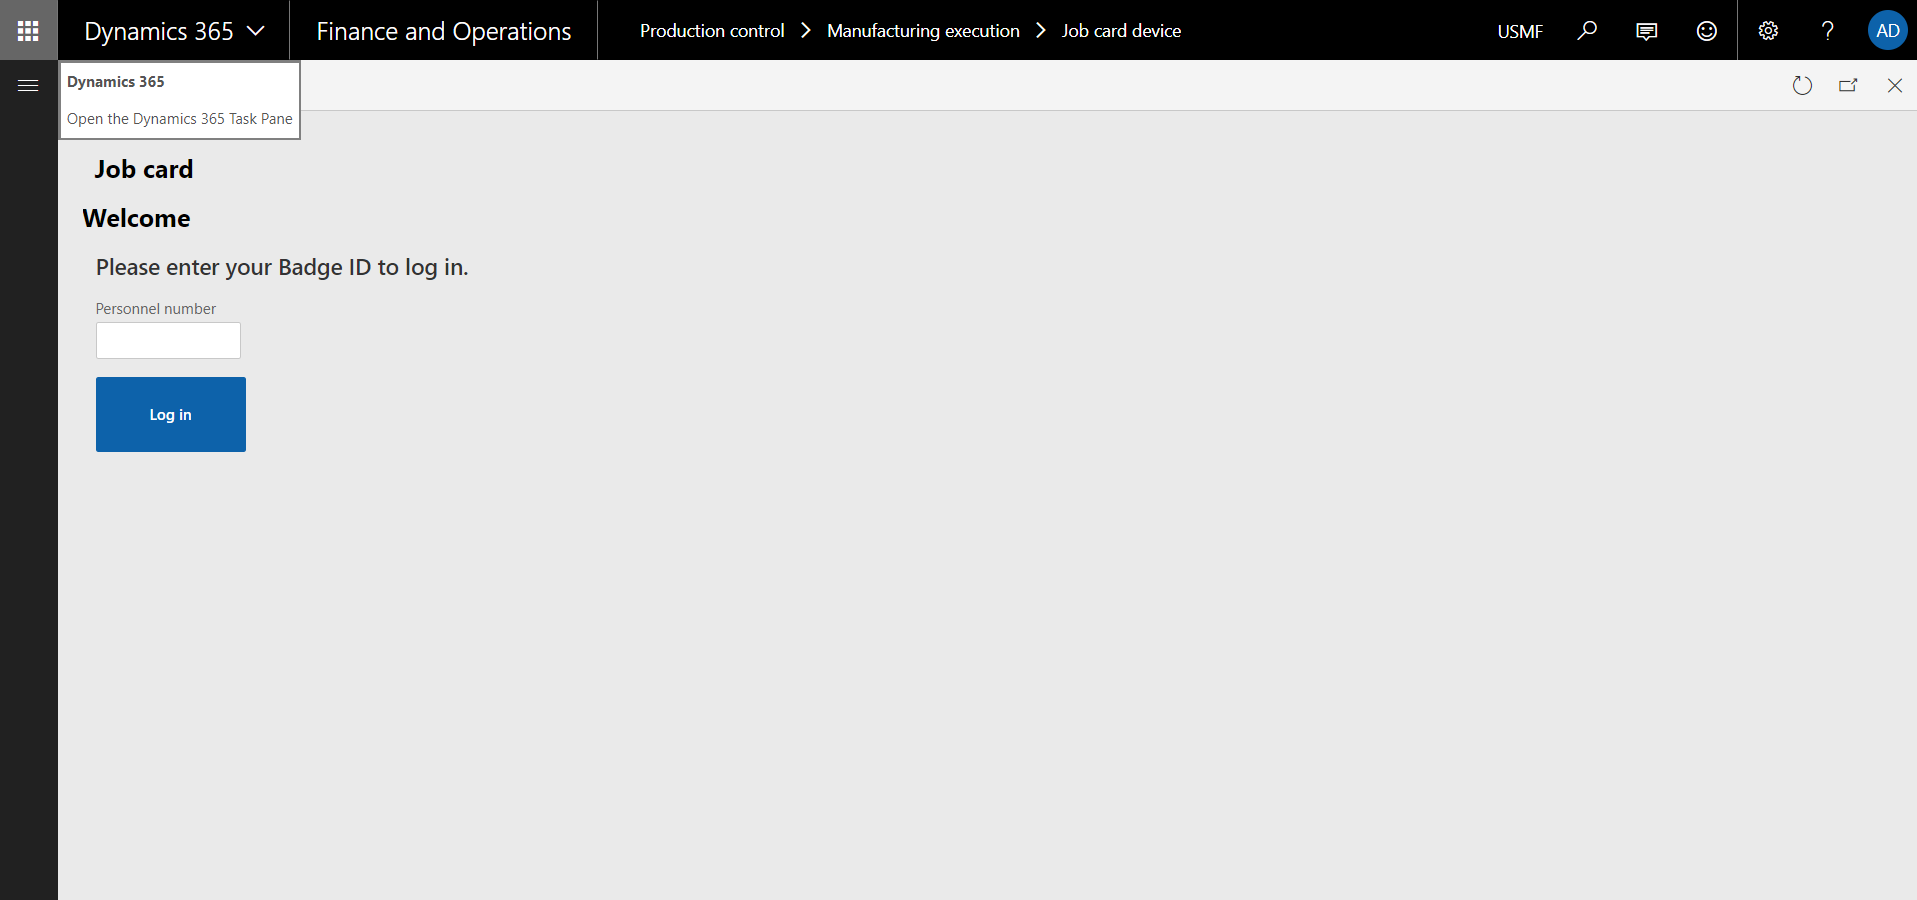
\includegraphics[width=0.8\textwidth]{img/d365productionControl3.png}
    \caption{Login-scherm Job Card Device module}
\end{figure}

Eens ingelogd komt de gebruiker dan in de Job Card Device module terecht (zie onderstaande figuur). Dit is de effectieve module waar dit onderzoek zich op zal toespitsen. De opzet is niet om de volledige module te dupliceren d.m.v. een bot, maar slechts enkele delen. Het is immers voldoende om die specifieke delen te behandelen, om aan te kunnen tonen dat een chatbot gemaakt in het MS Bot Framework in staat is om CRUD-operaties uit te voeren in D365FO. 
\begin{figure}[h]
    \centering
    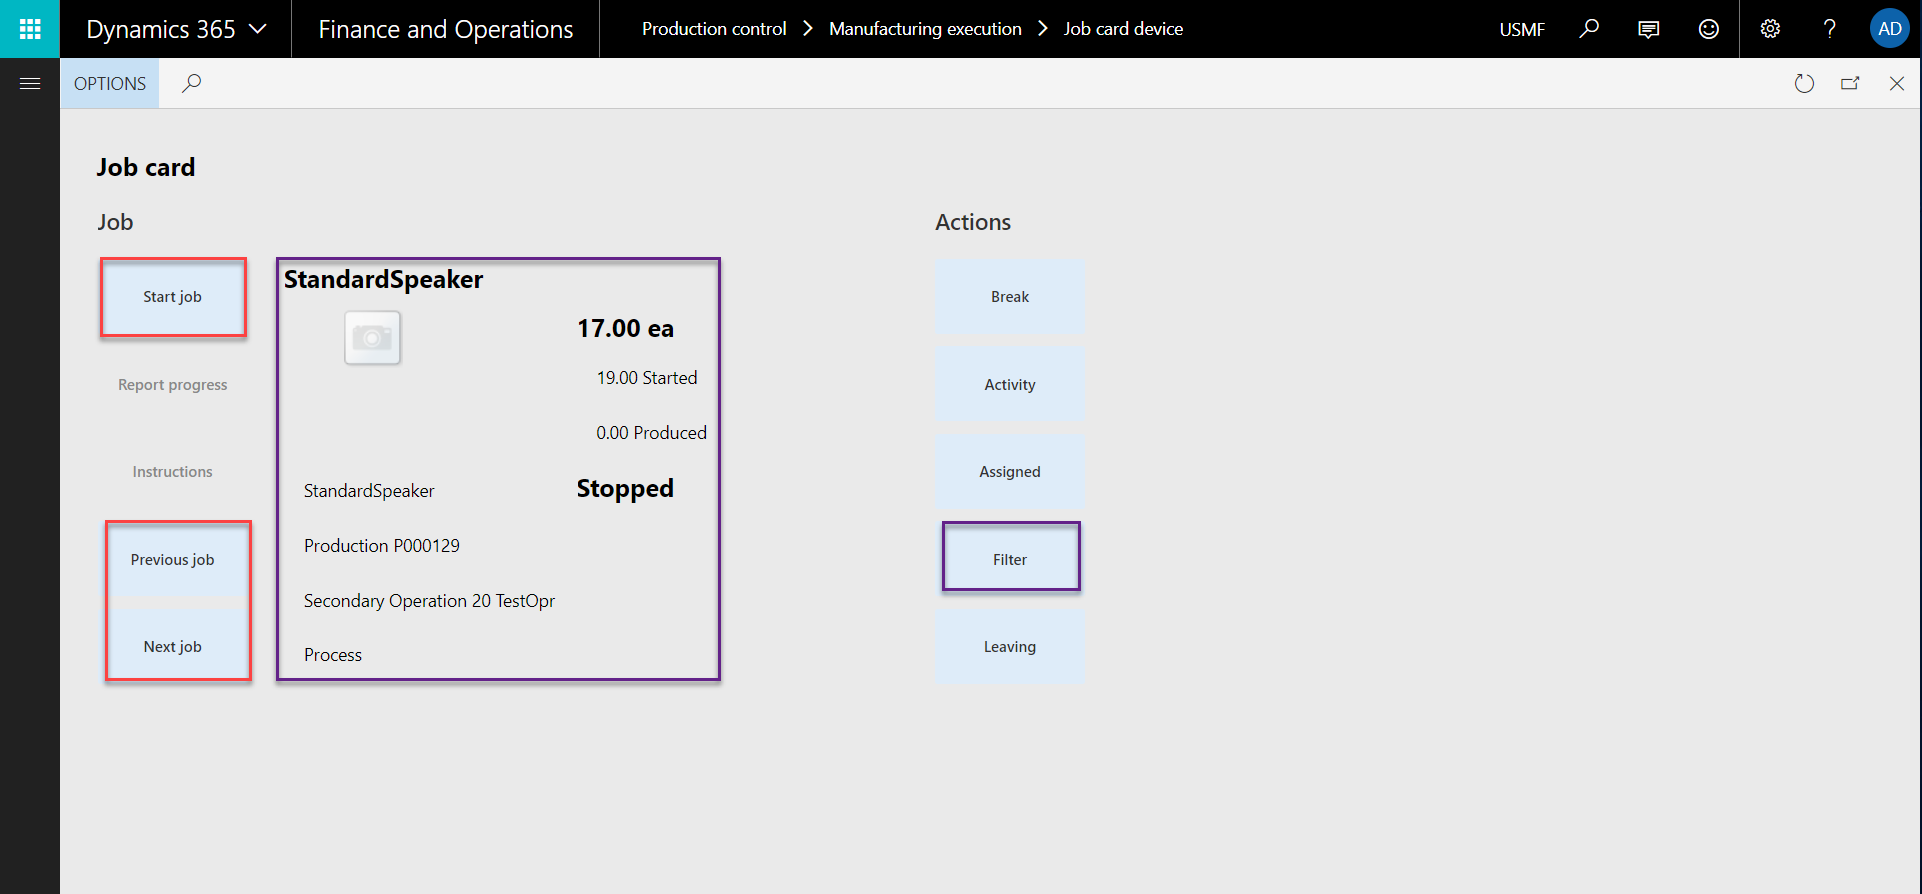
\includegraphics[width=0.8\textwidth]{img/d365productionControl4.png}
    \caption{Job Card Device module}
\end{figure}
Indeling scherm: De linkerzijde (zie rode kaders) omvat functionaliteiten die van toepassing zijn op een productie order. De knoppen aangeduid met een kader zullen in de chatbot verwerkt worden. Zo zal het dus mogelijk zijn om een job te starten (of stoppen, indien van toepassing), en om te navigeren tussen verschillende productie orders. De paarse kaders zullen ook verwerkt worden, namelijk in die zin dat het ook mogelijk zal zijn om informatie te zien over een productie order. Aanvullend zal er in de chatbot ook per productie order een bill of materials getoond worden. Dit was een extra requirement van de opdrachtgever (delaware), want een BOM is immers zeer relevante informatie voor een productiemedewerker. 


\section{Proof of concept}
Bij het onderzoek werd eerst een functionele analyse gemaakt op maat van het beoogde proof of concept. Allereerst werd hiervoor een user story opgemaakt om de scope van het onderzoek te bepalen. In onderstaande afbeelding ziet men een visuele representatie van het BPMN diagram. Voor een afbeelding op ware grootte kunnen de bijlagen geraadpleegd worden. 

\begin{figure}[h]
    \centering
    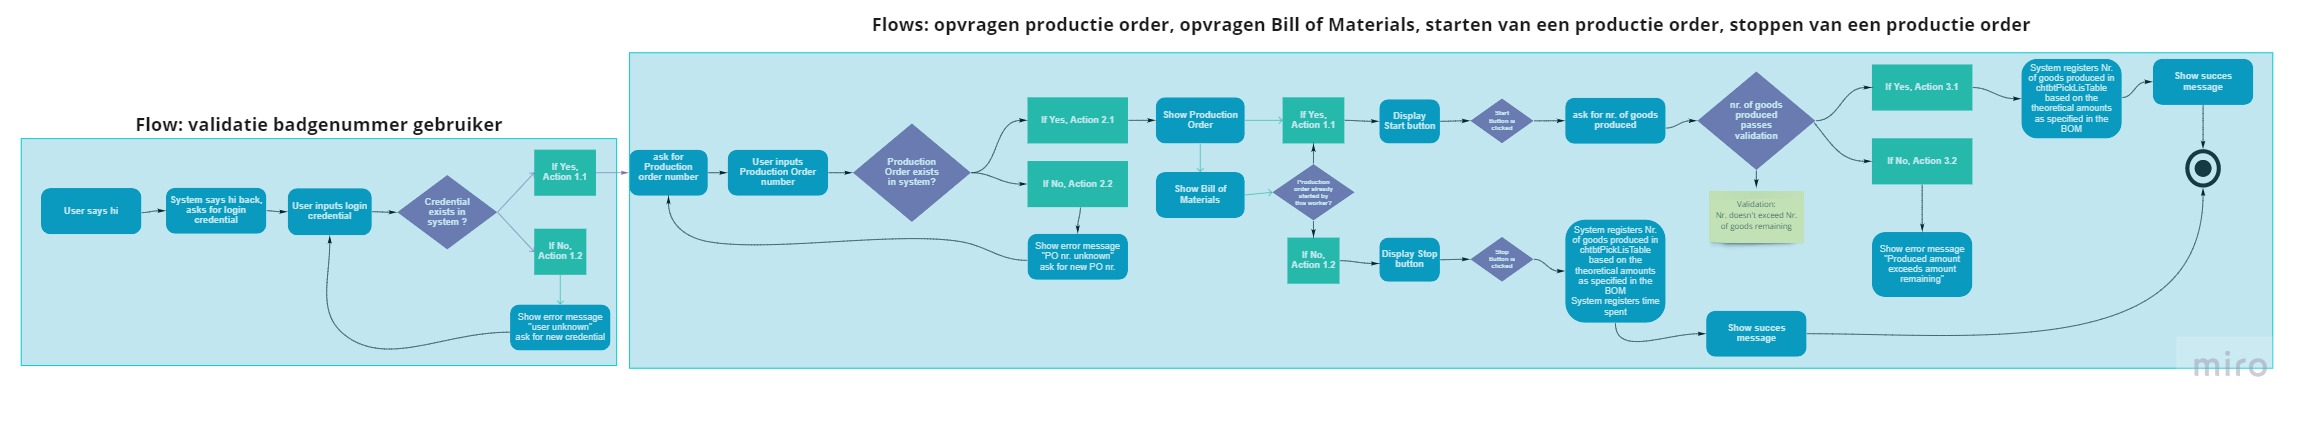
\includegraphics[width=1\textwidth]{img/HappyFlows.jpg}
    \caption{Business Process Model and Notation diagram POC }
\end{figure}

Enkele belangrijke opmerkingen: 
Het linkerdeel van het BPMN omvat must-have 5 (zie functionele requirements hieronder). Van zodra deze stap voldaan is kan de gebruiker acties uitvoeren in de chatbot, en niet eerder. Deze stap zal dus recurrent voorkomen bij alle functionaliteiten van de bot.

Verder zullen er er ook nog andere functionaliteiten in zitten die niet in het BPMN gedefinieerd zijn. Voorbeelden hiervan zijn nice to haves 3 en 4. Aangezien de flows voor deze functionaliteiten uit zéér weinig stappen bestaan, en dus in enige mate triviaal zijn. Daarom werd het opstellen van flows voor deze stappen als buiten de scope van dit onderzoek beschouwd. 

\subsubsection{functionele requirements}

Must haves:
\begin{enumerate}
    \item Er wordt een proof-of-concept gebouwd in het Microsoft Bot Framework. 
    \item Bovengenoemde bot gebruikt LUIS voor het interpreteren van natuurlijke zinnen naar commando's. 
    \item Ook moet de bot gepaste CRUD operaties kunnen uitvoeren in D365FO.
    \item De gebruiker kan inloggen adhv een badgeID (zonder deze badgeID kan de gebruiker niks doen. Validatie: badgeID bestaat in D365FO.)
    \item Eens ingelogd kan de gebruiker een aantal acties beginnen die voor hem van toepassing zijn:  
    \subitem De gebruiker kan een productieorder bekijken (titel, hoeveelheid en productieordernummer).
    \subitem De gebruiker kan de bill of materials zien van een productieorder (verschillende onderdelen, hoeveelheid en hoeveelheid per series)
    \subitem De gebruiker kan een productieorder starten. Hiervoor moet hij eerst een hoeveelheid invullen (validatie: hoeveelheid is kleiner of gelijk aan de resterende hoeveelheid)
    \subitem De gebruiker kan een productieorder stoppen (validatie: dit is enkel mogelijk als de gebruiker deze actie heeft gestart.) 
    
\end{enumerate}

Nice to haves:
\begin{enumerate}
    \item De gebruiker kan aan de hand van spraakherkenning communiceren met de bot.
    \item De gebruiker kan aan de hand van stemherkenning herkend worden door de bot, waardoor inloggen met badgeID niet langer noodzakelijk is
    \item De gebruiker kan aan de hand van een help-menu bekijken wat zijn opties zijn (welke stappen hij kan uitvoeren d.m.v. de bot)
    \item De gebruiker kan een overzicht zien van alle presentatie-mogelijkheden binnen de bot. Deze nice to have is louter voor presentatie doeleinden bestemd. Zo moet het mogelijk kunnen zijn om te raadplegen welke soorten informatie, en in welke vorm, allemaal raadpleegbaar zijn binnen de bot (foto's, video's, hyperlinks, etc.)
\end{enumerate}

Enkele belangrijke opmerkingen:
De focus voor dit onderzoek ligt niet op het coderen van zo veel mogelijk functionaliteiten, aangezien dit na de eerste keer veel repetitief werk met zich meebrengt. Het werd daarom als voldoende beschouwd door de opdrachtgever (delaware) wanneer er duidelijk vastgesteld kon worden dat er communicatie tussen D365FO en de bot mogelijk is (zie must have 3). Later in dit onderzoek zal samengevat worden wat de aangeraden stappen en best-practices hiervoor zijn.  Er zal daarom meer toegespitst worden op de werkwijze, en onder andere de voor- en nadelen. 

Tenslotte kunnen bovenstaande functionele requirements samenvattend weergegeven worden in volgende user stories: 

\begin{figure}[h]
    \centering
    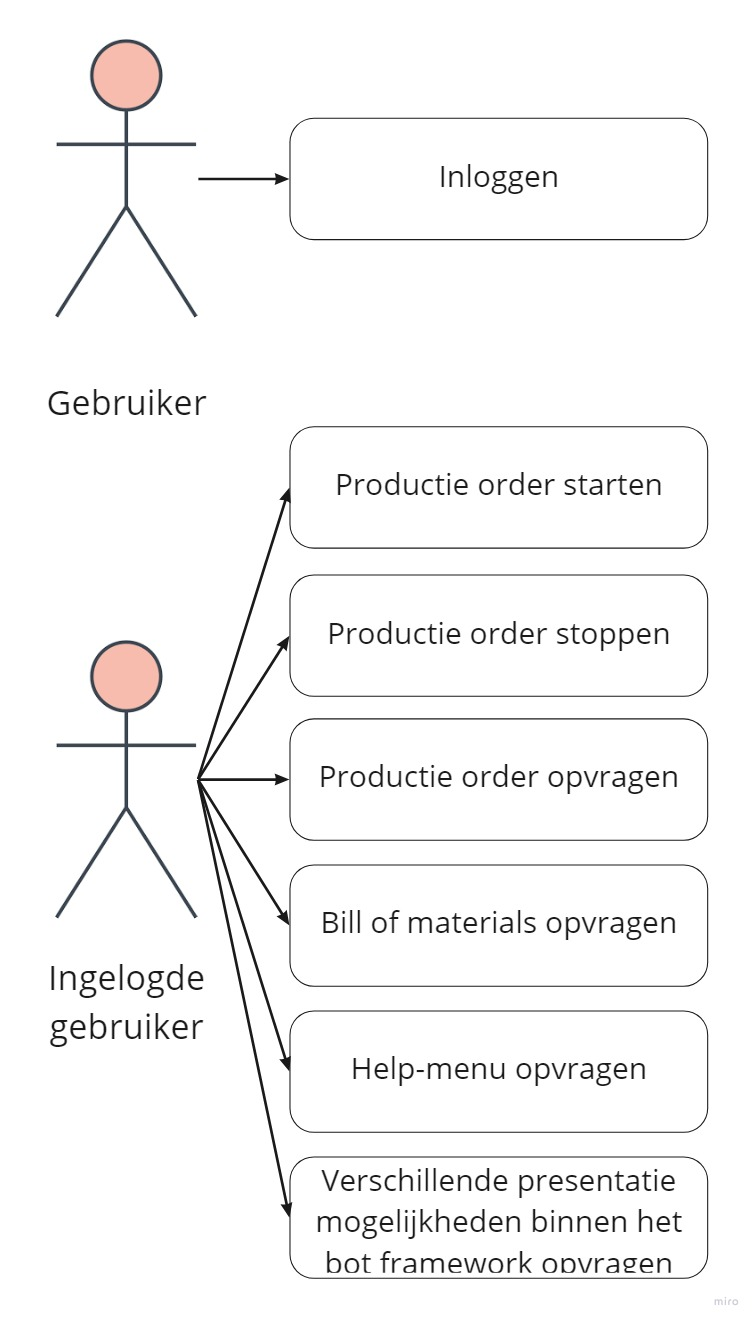
\includegraphics[width=0.32\textwidth]{img/UserStories.jpg}
    \caption{User stories POC }
\end{figure}


 

    %%=============================================================================
%% Technische Analyse
%%=============================================================================
\chapter{Technische Analyse}
\label{ch:technischeanalyse}

\section{Architectuur}
Voor het proof of concept zullen 3 applicaties worden gemaakt:
\begin{enumerate}
    \item D365FO applicatie met eigen model ('chtbt')
    \item C\# .NET webapplicatie voor authenticatie
    \item Implementatie in het MS Bot Framework
\end{enumerate}
\begin{figure}[h]
    \centering
    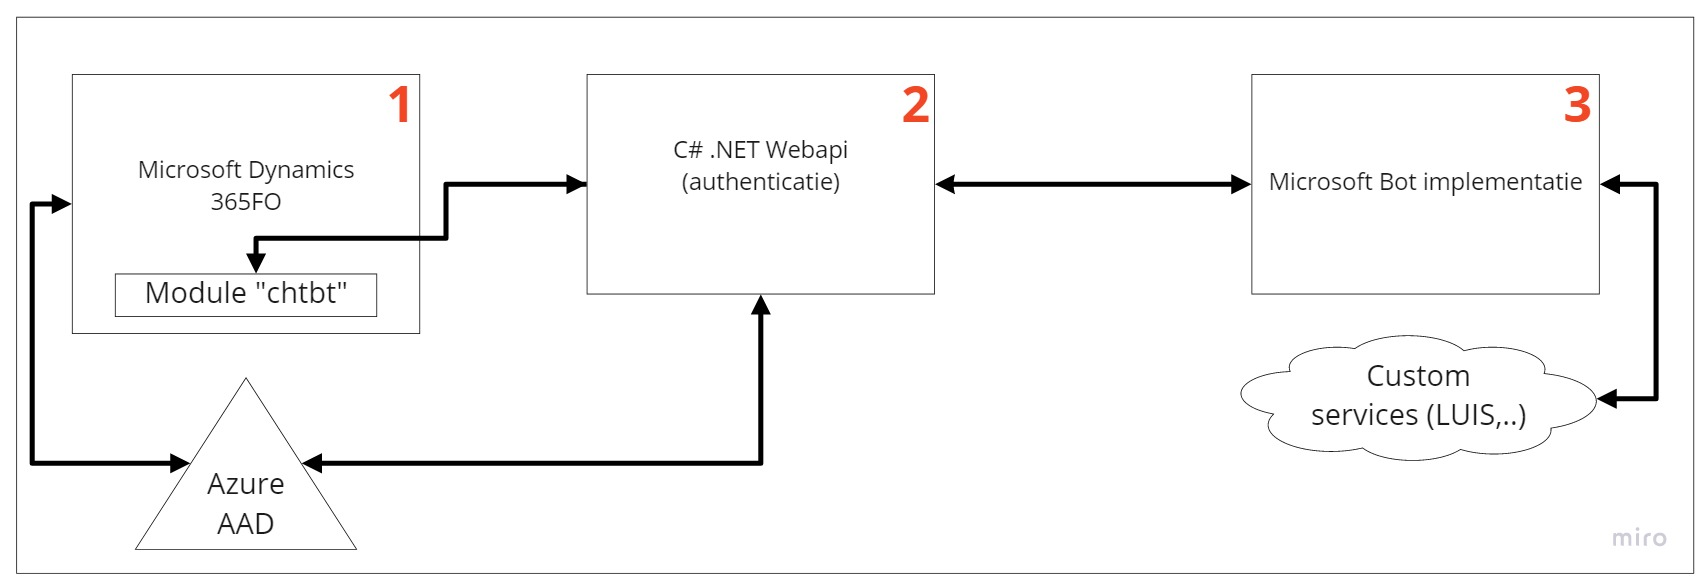
\includegraphics[width=1\textwidth]{img/ApplicatieArchitectuur}
    \caption{Applicatie architectuur}
\end{figure}
De eerste applicatie dient voor het programmeren van custom services binnen D365F0. Hiervoor zal een apart model gebouwd worden, genaamd 'chtbt' (afkorting voor chatbot). Binnen deze applicatie zal bestaande logica uit D365FO gebruikt, en beschikbaar gesteld worden d.m.v. een webservice. 

De tweede applicatie zal vervolgens connecteren met de eerste, en als communicatiemiddel dienen tussen de eerste en de derde applicatie. De reden dat hiervoor een aparte webapplicatie werd gebouwd is om de scheiding van taken en verantwoordelijkheden duidelijk af te bakenen per applicatie. Zo zal het authenticatiegedeelte (zie later) in deze omvat worden om gevoelige informatie (verbindingssleutels Azure, etc.) te verbergen voor de buitenwereld. 

Tenslotte zal uiteraard ook een chatbot gebouwd worden. Als deze dan wilt communiceren met D365FO om bepaalde CRUD-operaties uit te voeren, hoeft het enkel requests te versturen naar de authenticatie applicatie.

\section{Ontwikkel omgeving}
De ontwikkeling van het POC gebeurt volledig in de cloud, en dit op een Remote Desktop die draait op Lifecycle Services van Microsoft. Dit is een portaal waar meerdere mensen kunnen samenwerken, en dat de gebruiker assisteert in het beheren van de applicatie lifecycles van de verschillende D365FO implementaties.
Een schematische voorstelling:

\begin{figure}[H]
    \centering
    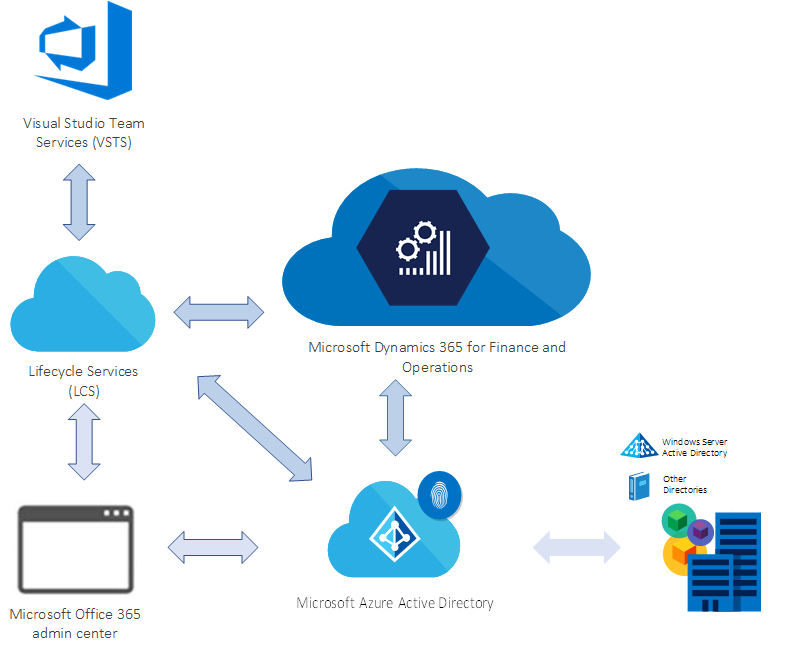
\includegraphics[width=0.8\textwidth]{img/lcsCloudArchitecture.png}
    \caption{Microsoft Lifecycle Services cloud architectuur}
\end{figure}

Aangezien dit proof of concept veel webrequests omvat, wordt er voor gekozen om deze eerst via de localhost te ontwikkelen. In een volgende stap zullen deze dan gehost worden. 

\section{Demo omgeving}
Wat betreft demo's van het poc zullen deze steeds 100\% in-cloud uitgevoerd worden. Dit wil zeggen dat alledrie de applicaties gehost zullen worden op hun respectievelijke webadressen, en de bot dus van eender waar bereikbaar, en bruikbaar is. 

De webadressen hiervoor zijn 
Insert finale webadressen
%%TODO 

\section{Authenticatie}
De authenticatie tussen Dynamics 365FO en de chatbot vereiste een aparte applicatie. Dit omdat de authenticatie volledig via Azure AAD verloopt. De authenticatie app werd geregistreerd binnen de D365FO Azure AAD applicaties (in D365FO: dashboard -> Azure Active Directory Applications). In D365FO ziet dit er als volgt uit: 
\begin{figure}[H]
    \centering
    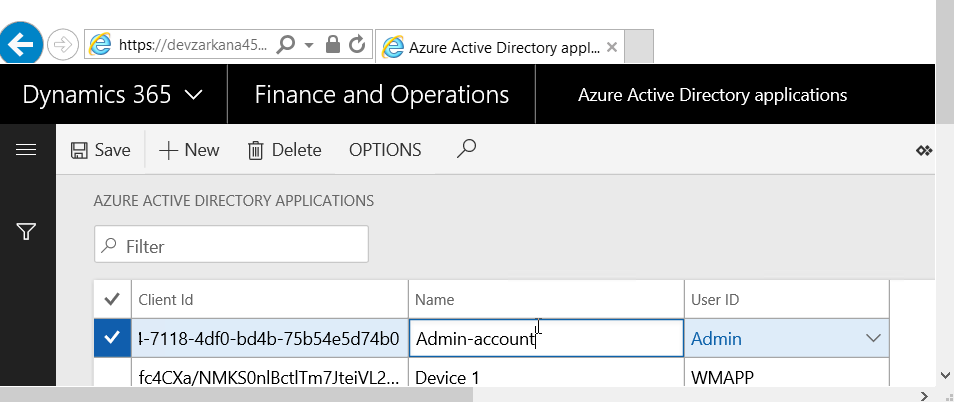
\includegraphics[width=1\textwidth]{img/impersination.png}
    \caption{Microsoft Lifecycle Services cloud architectuur}
\end{figure}
Nadat dit gebeurd is, kan er geconnecteerd worden met D365FO van buitenaf adhv. impersination. 
Dit wil zeggen dat wanneer iemand van buitenaf wilt inloggen op een d365FO omgeving, deze eerst moet inloggen op Azure om een Authorization Token te ontvangen. Vervolgens kan de gebruiker dan toegang aanvragen aan de resource (D365FO), om zo een Acces Token te kunnen bekomen. Als deze werd toegekend kan de Acces Token meegestuurd worden met alle volgende requests naar D365FO. Deze zal immers aan de Dynamics kant gevalideerd worden om dan toegang toe te kennen of te weigeren naargelang de situatie die zich voordoet. In onderstaande afbeelding wordt dit proces schematisch samengevat.

\begin{figure}[H]
    \centering
    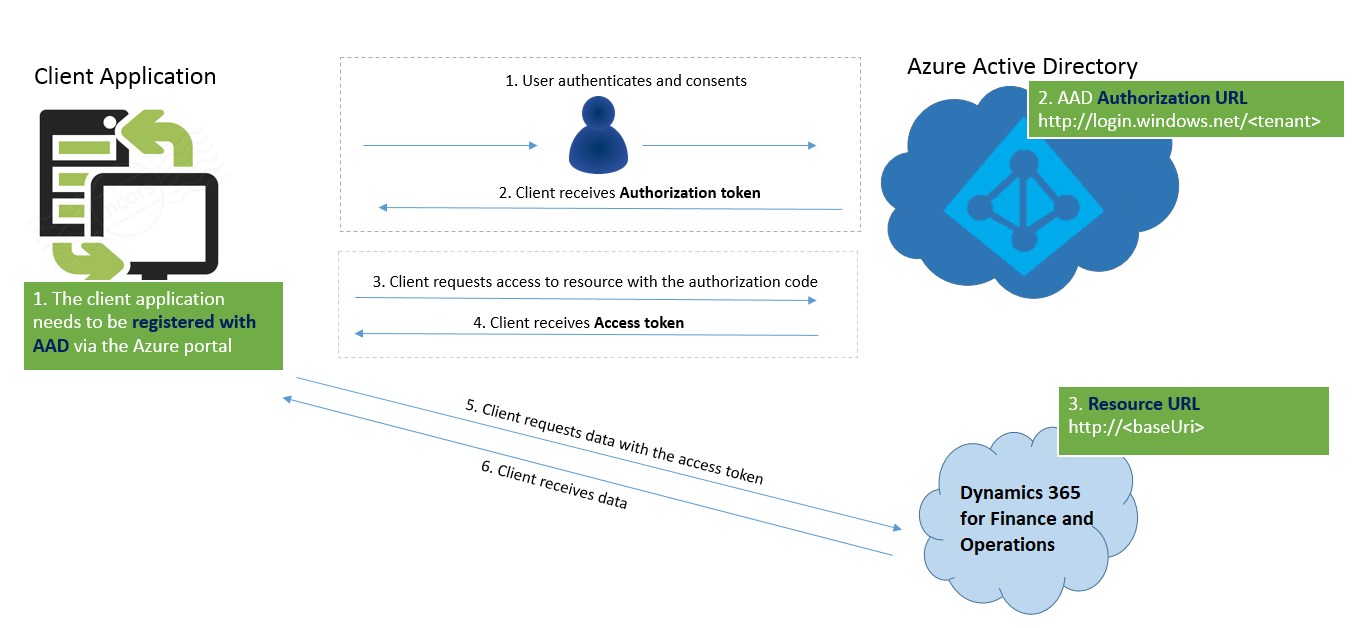
\includegraphics[width=1\textwidth]{img/aadAuthenticationArchitecture.png}
    \caption{D365FO authenticatie mbv Azure Active Directory}
\end{figure}
\subsection{Azure resources}
op het einde
\section{Data model}
Binnen D365FO zullen custom klassen en methodes gebruikt worden bovenop de reeds bestaande. De reden hiervoor is om op efficiënte manier informatie te kunnen versturen in webrequests. De bestaande klassen in D365FO zou een vorm van overkill zijn, omdat deze heel veel data bevatten die niet relevant is voor het poc. Deze klassen zullen vervolgens geserialiseerd verstuurd worden als JSON-objecten. 

\subsection{Json 2 Csharp}
De in D365FO (X++) geïmplementeerde klassen zullen vervolgens ook nodig zijn in de authenticatie app (C\#). Dit zodat de geserialiseerde JSON objecten gedeserialiseerd kunnen worden in C\# objecten. Hiervoor kan men er voor kiezen om alles dubbel te programmeren, wat dus ook dubbel werk betekent. Een andere optie is echter om de JSON strings te gebruiken voor de conversie. Hier zijn verschillende sites en tools voor, waarvan Json2Csharp.com een voorbeeld is. 
In onderstaande afbeelding wordt geïllustreerd hoe dit in zijn werk gaat. De geserialiseerde JSON string kan integraal geplakt worden, waarna de tool automatisch C\# klassen zal creëren die op hun beurt slechts gekopieerd en geplakt moeten worden in een nieuwe lege C\# klasse. 
\begin{figure}[H]
    \centering
    \includegraphics[width=1\textwidth]{img/json2Csharp.png}
    \caption{Json2Csharp voorbeeld}
\end{figure}

\section{UML}
    %%=============================================================================
%% Methodologie
%%=============================================================================

\chapter{\IfLanguageName{dutch}{Methodologie}{Methodology}}
\label{ch:methodologie}

%% TODO: Hoe ben je te werk gegaan? Verdeel je onderzoek in grote fasen, en
%% licht in elke fase toe welke stappen je gevolgd hebt. Verantwoord waarom je
%% op deze manier te werk gegaan bent. Je moet kunnen aantonen dat je de best
%% mogelijke manier toegepast hebt om een antwoord te vinden op de
%% onderzoeksvraag.

\section{Proof of Concept}
\subsection{MS Dynamics 365FO}
Voor de Dynamics 365 implementatie werd een eigen module gebouwd. Een module kan volgens \textcite{Microsoft2019} beschouwd worden als een verzameling van elementen binnen MS Dynamics 365. 

Voor dit onderzoek werd gekozen voor module naam `chtbt'. In onderstaande figuur wordt een overzicht weergegeven van alle elementen waaruit de module bestaat. 

\subsubsection{Custom klassen}
Daar de voorgebouwde klassen in MSD365FO enorm veel data en logica bevatten, werd er voor gekozen om ook eigen klassen te maken. Dit werd gedaan adhv Table-extensions. De grootste motivatie hiervoor was dat die klassen (productieorder en bill of materials) ook serialiseerbaar moesten zijn om te kunnen versturen via web requests. Het is daarom niet verstandig om gigantische klassen te gaan serialiseren en versturen wanneer er slechts een fractie van de verstuurde gegevens nodig zijn. 

Ook was het nodig om deze klassen langs de client-kant (chatbot) te kunnen deserialiseren om CRUD-operaties mogelijk te maken. De deserialisatie werd geautomatiseerd, in die zin dat er gebruik werd gemaakt van Json2Csharp (zie 6.5.1). 

\subsubsection{Custom services}
Eens het datamodel gebouwd is, moeten de nodige methodes uiteraard beschikbaar zijn vanuit een third-party applicatie zoals de chatbot. Om dit te bewerkstelligen heeft men enkele opties (per \textcite{Microsoft2019a})

\begin{itemize}
    \item Custom Services
    \item OData Service
\end{itemize}

\textbf{OData Service:}\\ 
Deze manier van werken kan per \textcite{Microsoft2019b} gedefineerd worden als: 
een standaard protocol voor het creëren en consumeren van data. Het doel hiervan is om een standaard manier van werken aan te bieden die gebaseerd is op het REST protocol voor het creëren, lezen, updaten en deleten van data binnen D365FO. Ook maakt de service gebruik van JSON voor het versturen van informatie. 

In de werkelijkheid komt het erop neer dat men vanuit third party apps queries kan uitvoeren en versturen naar D365FO. Een voorbeeld hiervan kan geraadpleegd worden op onderstaande afbeeldingen.

\begin{figure}[H]
    \centering
    \includegraphics[width=1\textwidth]{img/ODataExample}
    \caption{data creatie voor een create operatie adhv OData binnen D365FO \cite{Lanssens2018}}
    
\end{figure}

\begin{figure}[H]
    \centering
    \includegraphics[width=1\textwidth]{img/ODataExample2}
\caption{webrequest creatie en versturing voor een create operatie adhv OData binnen D365FO \cite{Lanssens2018}}
\end{figure}

\textbf{Custom Services}\\
Voor dit onderzoek werd er voor gekozen om niet gebruik te maken van Odata Servies, maar van Custom Services. Dit wil zeggen dat men langs D365FO's kant zelf services gaat definiëren, en deze beschikbaar gaat stellen via hun eigen endpoint. Deze manier van werken is iets overzichtelijker wanneer er van de buitenwereld gebruikt wordt gemaakt van custom methodes binnen D365FO die een of meerde parameters verwachten. In D365FO hoeft men enkel te definiëren welke parameters binnenkomen, en deze te verwerken, Terwijl in de third party app (bot) slechts de juiste endpoints moeten worden aangesproken samen met de nodige parameters. 

Een handleiding in detail van hoe dit werd gerealiseerd kan worden teruggevonden in de bijlagen (bijlage D).


\subsection{Authenticatie Applicatie}
Zoals gezegd werd er doelbewust gekozen om het authenticatiegedeelte te encapsuleren in een aparte applicatie. Dit om gevoelige informatie, zoals connectiesleutels etc., te kunnen verbergen van de buitenwereld. 

Maar verder is deze manier van werken interessant, omdat meerdere bots deze zouden kunnen gebruiken, maar ook andere third-party apps (zoals bv. een mobiele app) zouden in principe dankzij deze tussenapplicatie kunnen connecteren met D365FO. 

\subsection{MS Bot Framework implementatie}
\subsubsection{Bot zelf}
Dankzij Azure is het aanmaken van een nieuwe bot relatief eenvoudig. Zo zal de portaal automatisch alle benodigde resources aanmaken en configureren voor de nieuw aangemaakte bot.\\

Voor dit onderzoek werd gekozen voor een Web App Bot (template: Basic Bot) van SDK 4. Dit is de meest recente (2019), en implementeert LUIS al gedeeltelijk. Dit is een ideaal vertrekpunt voor een nieuwe chatbot die natuurlijke taal verwerkt en beantwoordt met gepaste verlopen specifiek per casus. 

Een handleiding in detail van hoe dit werd gerealiseerd kan worden teruggevonden in de bijlagen (bijlage B).

Dankzij het waterval-principe 

\subsubsection{NLP}
Uiteraard is één van de kerncomponenten van een chatbot natural language processing (NLP). In het Microsoft Bot Framework wordt LUIS gebruikt als engine om natuurlijke taal om te zetten naar bruikbare commando's die elk hun eigen invulling vereisen.\\ 

\rightline{\textbf{Werking}}
Voor de werking rust LUIS op 2 kernbegrippen. Intenties enerzijds, en Entiteiten anderzijds. Intenties worden gebruikt om aan te duiden wat de gebruiker wilt doen. Zo zal een chatbot anders reageren als een gebruiker wilt weten hoelaat het is, dan indien hij het weer voor die dag zou opvragen.\\
\rightline{Intenties:}\\
Deze component wordt gebruikt om een bot op te delen in verschillende functionaliteiten. Elke intentie zal zijn eigen vervolg geven aan het bericht van de gebruiker. Zo zal het verloop bij de intentie `GeefWeer' anders reageren dan bij de intentie 'GeefProductieOrders'. 

Wanneer men een LUIS app maakt kan men intenties opgeven, en hier voorbeeldzinnen aan toevoegen. De service zal dan automatisch op basis van de voorbeeldzinnen het model trainen (Machine Learning). Hierna kunnen zinnen naar LUIS verstuurd worden, en LUIS zal dan voor elke zin een score gaan berekenen per intentie. Met andere woorden: hoe groot is de kans dat de gebruiker met zin 'x' intentie 'y' wil bereiken. De intentie die hier het hoogst op scoort zal gekozen worden, en vervolgens teruggestuurd worden. 
Op onderstaande figuur wordt een illustratief maar niet limitatief voorbeeld weergegeven. 

\begin{figure}[H]
    \centering
    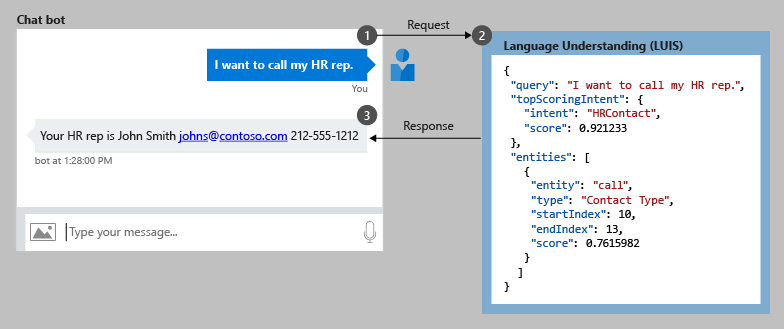
\includegraphics[width=1\textwidth]{img/LuisIntents}
\caption{voorbeeld van een LUIS respons \cite{Microsoft2019c}}
\end{figure}

\rightline{Entiteiten:}
Wanneer men NLP wil bereiken op een efficiënte manier, zal men ook enige notie moeten hebben van entiteiten. Onder deze term wordt alle bijkomende informatie, die van belang is, verzameld. Zo is het bijvoorbeeld niet enkel nodig om te weten dat een gebruiker het weer wil zien, maar ook van welke dag. Net zoals dat het niet enkel handig is om te weten dat de gebruiker een productie order wil bekijken, maar ook het productie order nummer in kwestie zal vereist zijn.
Ook hier treedt een vorm van artificiële intelligentie op. Zo zal LUIS immers automatisch herkennen of er entiteiten aanwezig zijn in een zin, en deze terugsturen met zijn antwoord. Uiteraard is dit niet vanzelfsprekend, en verwacht LUIS ook hier dat je de service eerst traint. Dit doet men door de nodige entiteiten te definiëren. Hiervoor heeft de developer verschillende keuzes. Zo is het mogelijk om een entiteit te definiëren aan de hand van patronen, reguliere expressies, composities, etc. \\
Op onderstaande figuur wordt weergegeven hoe een compositie eruit ziet. We zien dat er 3 entiteiten (number, PassengerClass en Travelclass) gedefinieerd zijn. Dankzij voorbeelden van elke entiteit en training is LUIS in staat de entiteiten te herkennen, en automatisch toe te voegen aan de compositie.

\begin{figure}[h]
    \centering
    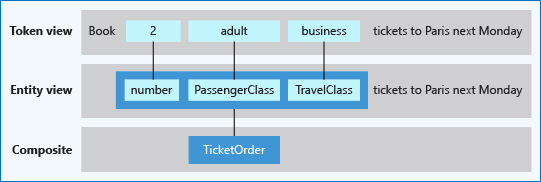
\includegraphics[width=0.8\textwidth]{img/LuisEntities}
    \caption{voorbeeld van LUIS entiteiten \cite{Microsoftd}}
    \end{figure}

Een handleiding in detail van hoe dit werd gerealiseerd voor deze poc kan worden teruggevonden in de bijlagen (bijlage C).

----------------------------------------------------------
\section{Onderzoek}
Aangezien het meten van onderzoeksvraag B nogal lastig is (Er zijn weinig meetbare parameters om dit te kunnen bevestigen/ontkrachten). Daarom werd er in dit onderzoek voor gekozen om een bevraging te doen naar de meningen van gebruikers. Voor het afnemen van de enquête werd er een demo en uitleg gegeven bij het doorlopen van 1 funtionaliteit (productieorder opzoeken \& starten). Vervolgens werd een bevraging gedaan naar beide systemen op vlak van: 

\begin{itemize}
    \item gebruiksvriendelijkheid
    \item eenduidigheid
    \item tijdverlies
\end{itemize}

\subsection{Vragenlijst}
onder deze noemers wordt het volgende verstaan:

\textbf{eenduidigheid}\\
Alles is duidelijk omschreven, er heerst geen onduidelijkheid over wat welke knop/stap teweeg zal brengen.\\

\textbf{gebruiksvriendelijkheid}\\
Het systeem voelt intuïtief en robuust aan. De gebruiker heeft steeds het gevoel dat hij de controle heeft.\\

\textbf{tijdverlies}\\
De gebruiker moet lang wachten tussen clicks in, het duurt trager dan dat het zou mogen duren.

Zo werd er gevraagd om steeds een score te geven van 1-5. Elke gebruiker heeft dus 6 scores opgegeven. Tenslotte werd er ook bij elk systeem (D365 vs chatbot) gevraagd of er opmerkingen/feedback waren.
in onderstaande figuur vind men een overzicht terug van de gebruikers, en hun scores.  


\subsection{Resultaten}
Op figuur 7.1 kan een overzicht worden teruggevonden van de onderzoeksresultaten. Voor meer info over de enquête kunnen de bijlagen geraadpleegd worden (bijlage f). 
\begin{table}[]
    \begin{tabular}{llll}
        \cline{1-2}
        \multicolumn{1}{|l|}{Gebruikers}                                   & \multicolumn{1}{l|}{aantal} &                              &                                                \\ \cline{1-2}
        \multicolumn{1}{|l|}{Met voorkennis D365FO (medewerkers delaware)} & \multicolumn{1}{l|}{14}     &                              &                                                \\ \cline{1-2}
        \multicolumn{1}{|l|}{Zonder voorkennis D365FO}                     & \multicolumn{1}{l|}{6}      &                              &                                                \\ \cline{1-2}
        \multicolumn{1}{|l|}{Totaal}                                       & \multicolumn{1}{l|}{20}     &                              &                                                \\ \cline{1-2}
        &                             &                              &                                                \\ \hline
        \multicolumn{1}{|l|}{\textbf{gemiddelden}}                         & \multicolumn{1}{l|}{D365FO} & \multicolumn{1}{l|}{Chatbot} & \multicolumn{1}{l|}{Verschil (D365FO-Chatbot)} \\ \hline
        \multicolumn{1}{|l|}{Gebruiksvriendelijkheid}                      & \multicolumn{1}{l|}{3.36}   & \multicolumn{1}{l|}{4.27}    & \multicolumn{1}{l|}{-0.93}                     \\ \hline
        \multicolumn{1}{|l|}{Eenduidigheid}                                & \multicolumn{1}{l|}{3.43}   & \multicolumn{1}{l|}{3.86}    & \multicolumn{1}{l|}{-0.43}                     \\ \hline
        \multicolumn{1}{|l|}{Tijdverlies}                                  & \multicolumn{1}{l|}{3.30}   & \multicolumn{1}{l|}{3.00}    & \multicolumn{1}{l|}{0.29}                      \\ \hline
    \end{tabular}
\caption{\label{tab:Overzicht bevraging Dynamics 365FO vs Chatbot}Overzicht bevraging Dynamics 365FO vs Chatbot}
\end{table}

\subsection{conclusie}
Men merkt al snel op dat de chatbot voor gebruiksvriendelijkheid bijna 1 punt (0.93) beter scoort dan Dynamics 365FO. Ook voor Eenduidigheid en tijdverlies presteert de chatbot respectievelijk 0,43 en 0.29 punten beter dan Dynamics. Alhoewel dit vrij aanzienlijk is op 20 bevragingen, moet men rekening houden met het aantal bevragingen. Verder blijft het een kwestie van meningen, en dus geen exacte wetenschap. 


    
    % Voeg hier je eigen hoofdstukken toe die de ``corpus'' van je bachelorproef
    % vormen. De structuur en titels hangen af van je eigen onderzoek. Je kan bv.
    % elke fase in je onderzoek in een apart hoofdstuk bespreken.
    %%%=============================================================================
%% Stakeholders
%%=============================================================================

\chapter{Stakeholders}
\label{ch:stakeholders}


\section{delaware}
\subsection{Algemeen}
delaware is een jonge consultancy firma die geavanceerde oplossingen op maat maakt voor, en diensten aanbiedt aan bedrijven die hun competitieve positie willen versterken op een houdbare manier. Zo zijn ze gespecialiseerd in het transformeren van hun klanten hun Finance, HR, Communicatie, en IT afdelingen. Dit varieert tussen implementaties op maat in vaak nieuwe technologieën, tot meedenken op strategische niveaus om hun brand te verbeteren. 
Sinds de herstructurering in 2005 zijn hun business activiteiten fors gegroeid. Zo telt delaware op de dag van vandaag meer dan 2000 werknemers, van 32 nationaliteiten, verspreid over 24 kantoren in 12 landen. In 2017 onderging het een naamsverandering, zo werd delaware Consulting uiteindelijk delaware. Dit toont hun engagement om aan te passen aan veranderende klantnoden en omstandigheden, die vaak de capaciteiten van een reguliere IT-consultancy firma overstijgen. Zo denkt delaware ook mee op de strategische en operationele niveaus.  
delaware steunt al sinds het prille begin op 3 pilaren. Allereerst Operational Excellence, hiermee bedoelt men dat ze op operationeel vlak, in de mate van het mogelijke, steeds zo efficiënt mogelijk te werk willen gaan, wat zich vaak uit in het verkennen van nieuwe technologieën en implementaties op maat. Ten tweede Business Insights, want technologie moet nu eenmaal als meerwaarde hebben dat de business waardevolle inzichten kan verwerven dankzij die technologie om met die inzichten aanpassingen te kunnen maken. Tenslotte is ook Customer Experience een pilaar, daar klanten de sleutel zijn voor elke firma. Deze 3 pilaren zijn sterk te herkennen wanneer men het heeft over de specialisaties van delaware, namelijk ERP-systemen, Business Intelligence en E-commerce. 
Als een van de leading partners van SAP en Microsoft beschikken ze over meerdere certificaten, zoals: Gold Certified Microsoft, Gold SAP, Gold Business Objects and Platinum OpenText partners.

\subsection{Vestigingen}
De dag van vandaag telt delaware 5 vestigingen in België, met als hoofdzetel de vestiging in Kortrijk. Dit omdat het bedrijf bewust omspringt met de behoeften van klanten, maar vooral van werknemers. 
Ook op globaal vlak deinst het bedrijf hier niet voor terug. Zo zijn veel van de internationale vestigingen strategisch gekozen om mee te groeien met hun klanten, en vooral hun internationale noden. 

\section{Microsoft}


\subsection{MS Bot Framework} 
Als de integratie tussen het Bot Framework en Dynamics 365 FO van dermate hoge kwaliteit is zal ook Microsoft hier voordeel uit putten. Zo zal hun ERP systeem een aanzienlijke toegevoegde waarde krijgen, dankzij hun eigen chatbot framework. Het is daarom niet onbelangrijk wat de uitslag en conclusie zal zijn van dit onderzoek voor Microsoft. 

\subsection{MS Azure} 
Aangezien het Bot Framework heel nauw verbonden is met Azure (zie volgende hoofdstukken), is ook het hosting platform in enige vorm stakeholder van dit onderzoek.
%te bespreken => 2e leven microsoft (erp, business2business, open-source,...)

    %%%=============================================================================
%% Projectplan
%%=============================================================================
\chapter{Projectplan}
\label{ch:projectplan}

\section{Projectplan}
    %%%=============================================================================
%% Stakeholders
%%=============================================================================

\chapter{Stakeholders}
\label{ch:stakeholders}


\section{delaware}
\subsection{Algemeen}
delaware is een jonge consultancy firma die geavanceerde oplossingen op maat maakt voor, en diensten aanbiedt aan bedrijven die hun competitieve positie willen versterken op een houdbare manier. Zo zijn ze gespecialiseerd in het transformeren van hun klanten hun Finance, HR, Communicatie, en IT afdelingen. Dit varieert tussen implementaties op maat in vaak nieuwe technologieën, tot meedenken op strategische niveaus om hun brand te verbeteren. 
Sinds de herstructurering in 2005 zijn hun business activiteiten fors gegroeid. Zo telt delaware op de dag van vandaag meer dan 2000 werknemers, van 32 nationaliteiten, verspreid over 24 kantoren in 12 landen. In 2017 onderging het een naamsverandering, zo werd delaware Consulting uiteindelijk delaware. Dit toont hun engagement om aan te passen aan veranderende klantnoden en omstandigheden, die vaak de capaciteiten van een reguliere IT-consultancy firma overstijgen. Zo denkt delaware ook mee op de strategische en operationele niveaus.  
delaware steunt al sinds het prille begin op 3 pilaren. Allereerst Operational Excellence, hiermee bedoelt men dat ze op operationeel vlak, in de mate van het mogelijke, steeds zo efficiënt mogelijk te werk willen gaan, wat zich vaak uit in het verkennen van nieuwe technologieën en implementaties op maat. Ten tweede Business Insights, want technologie moet nu eenmaal als meerwaarde hebben dat de business waardevolle inzichten kan verwerven dankzij die technologie om met die inzichten aanpassingen te kunnen maken. Tenslotte is ook Customer Experience een pilaar, daar klanten de sleutel zijn voor elke firma. Deze 3 pilaren zijn sterk te herkennen wanneer men het heeft over de specialisaties van delaware, namelijk ERP-systemen, Business Intelligence en E-commerce. 
Als een van de leading partners van SAP en Microsoft beschikken ze over meerdere certificaten, zoals: Gold Certified Microsoft, Gold SAP, Gold Business Objects and Platinum OpenText partners.

\subsection{Vestigingen}
De dag van vandaag telt delaware 5 vestigingen in België, met als hoofdzetel de vestiging in Kortrijk. Dit omdat het bedrijf bewust omspringt met de behoeften van klanten, maar vooral van werknemers. 
Ook op globaal vlak deinst het bedrijf hier niet voor terug. Zo zijn veel van de internationale vestigingen strategisch gekozen om mee te groeien met hun klanten, en vooral hun internationale noden. 

\section{Microsoft}


\subsection{MS Bot Framework} 
Als de integratie tussen het Bot Framework en Dynamics 365 FO van dermate hoge kwaliteit is zal ook Microsoft hier voordeel uit putten. Zo zal hun ERP systeem een aanzienlijke toegevoegde waarde krijgen, dankzij hun eigen chatbot framework. Het is daarom niet onbelangrijk wat de uitslag en conclusie zal zijn van dit onderzoek voor Microsoft. 

\subsection{MS Azure} 
Aangezien het Bot Framework heel nauw verbonden is met Azure (zie volgende hoofdstukken), is ook het hosting platform in enige vorm stakeholder van dit onderzoek.
%te bespreken => 2e leven microsoft (erp, business2business, open-source,...)

    %%%=============================================================================
%% Funcionele Analyse
%%=============================================================================

\chapter{Functionele Analyse}
\label{ch:funcioneleanalyse}


\section{Situatie as is}
\begin{figure}[h]
\centering
\begin{minipage}[t]{0.49\textwidth}   
    \includegraphics*[width=1\textwidth]{img/d365productionControl1}
    \caption{D365FO dashboard}
\end{minipage}
\begin{minipage}[t]{0.49\textwidth}
    \includegraphics*[width=1\textwidth]{img/d365productionControl2}
    \caption{Overzicht alle modules binnen D365FO}
\end{minipage}
\end{figure}
    
Dit onderzoek zal zich toespitsen op de Job Card Device module binnen D365FO. Op bovenstaande figuren ziet men screenshots uit het D365FO dasboard. Eens ingelogd ziet een gebruiker deze schermen, aangepast voor hem. Zo zal een productiemedewerker bijvoorbeeld aanzienlijk minder informatie beschikbaar hebben. De module Personnel Management is voor hem bijvoorbeeld niet van toepassing en bijgevolg zal de productiemedewerker deze niet zien. Dit geldt ook voor andere irrelevante modules en voor afzonderlijke menupunten binnen de schermen. Een productiemederwerker gaat bijvoorbeeld op een bepaald scherm 2 knoppen hebben, terwijl een manager er 20 gaat hebben.

Eens de gebruiker heeft genavigeerd naar de Production Control module zal hij kunnen kiezen voor de job card Device module. Deze module zal, gelijkaardig aan de chatbot, eerst vragen om in te loggen met zijn badgeID (zie onderstaand). Dit omdat het niet mogelijk (mag zijn) is om acties uit te voeren binnen de job card Device zonder ingelogd te zijn. 

\begin{figure}[H]
    \centering
    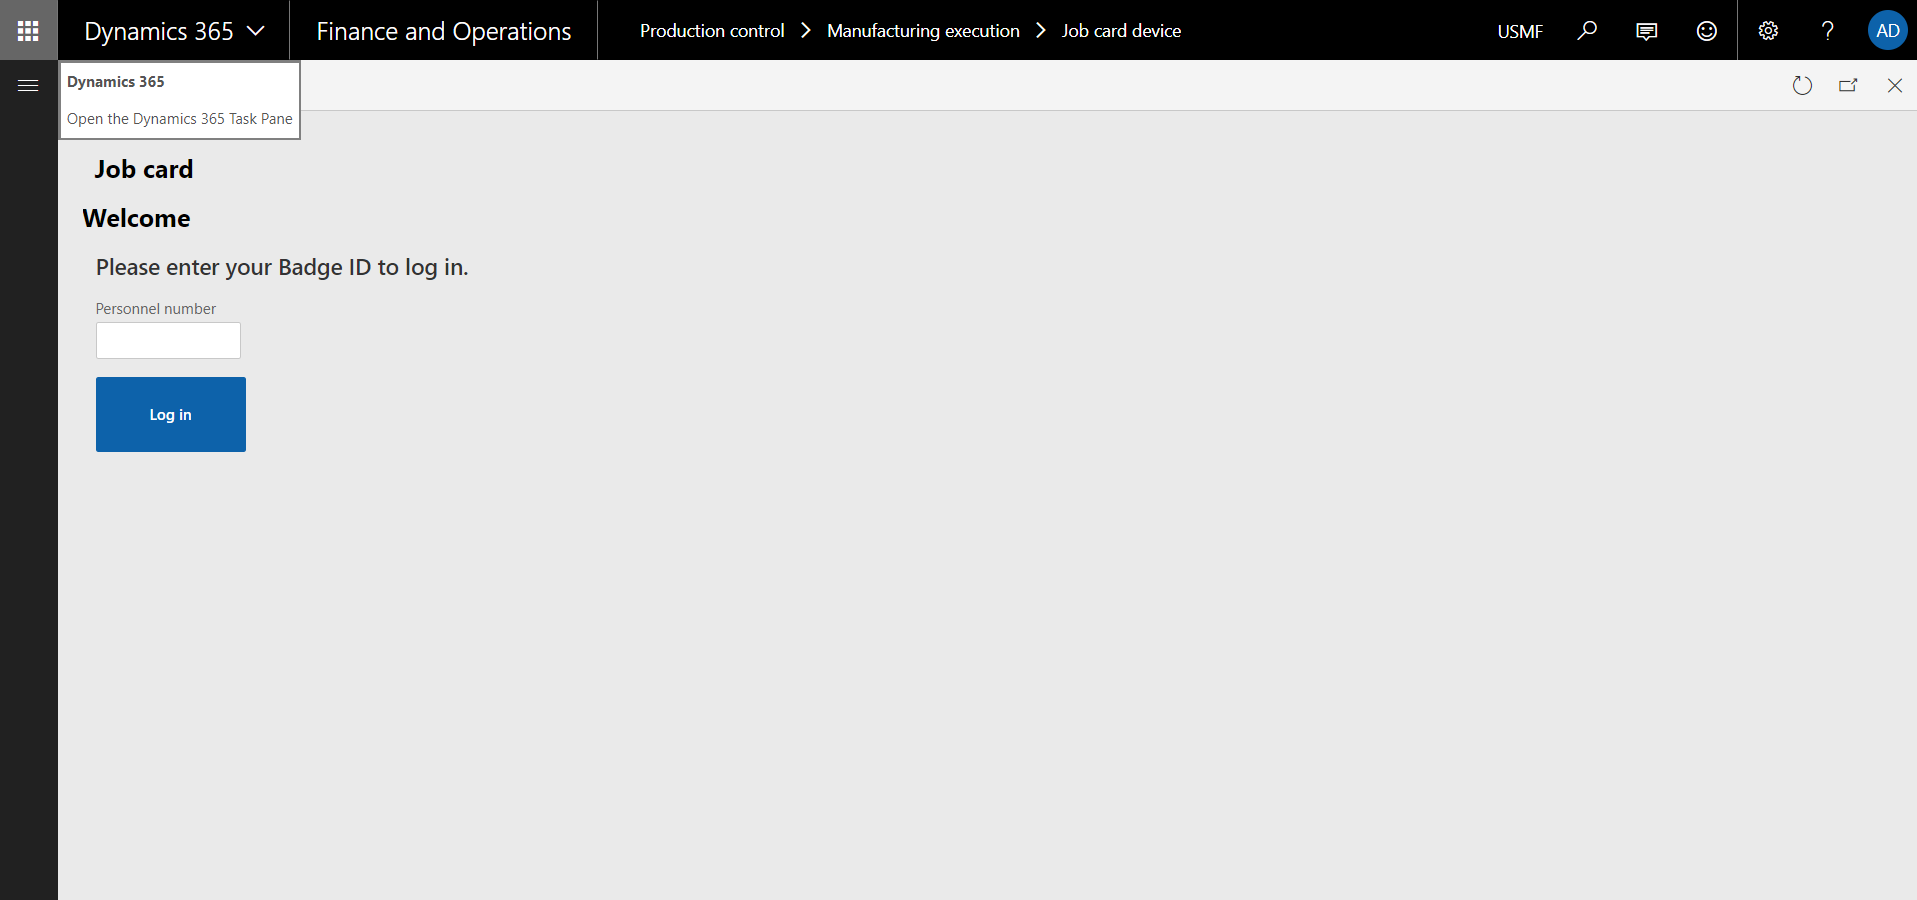
\includegraphics[width=0.8\textwidth]{img/d365productionControl3.png}
    \caption{Login-scherm Job Card Device module}
\end{figure}

Eens ingelogd komt de gebruiker dan in de Job Card Device module terecht (zie onderstaande figuur). Dit is de effectieve module waar dit onderzoek zich op zal toespitsen. De opzet is niet om de volledige module te dupliceren d.m.v. een bot, maar slechts enkele delen. Het is immers voldoende om die specifieke delen te behandelen, om aan te kunnen tonen dat een chatbot gemaakt in het MS Bot Framework in staat is om CRUD-operaties uit te voeren in D365FO. 
\begin{figure}[h]
    \centering
    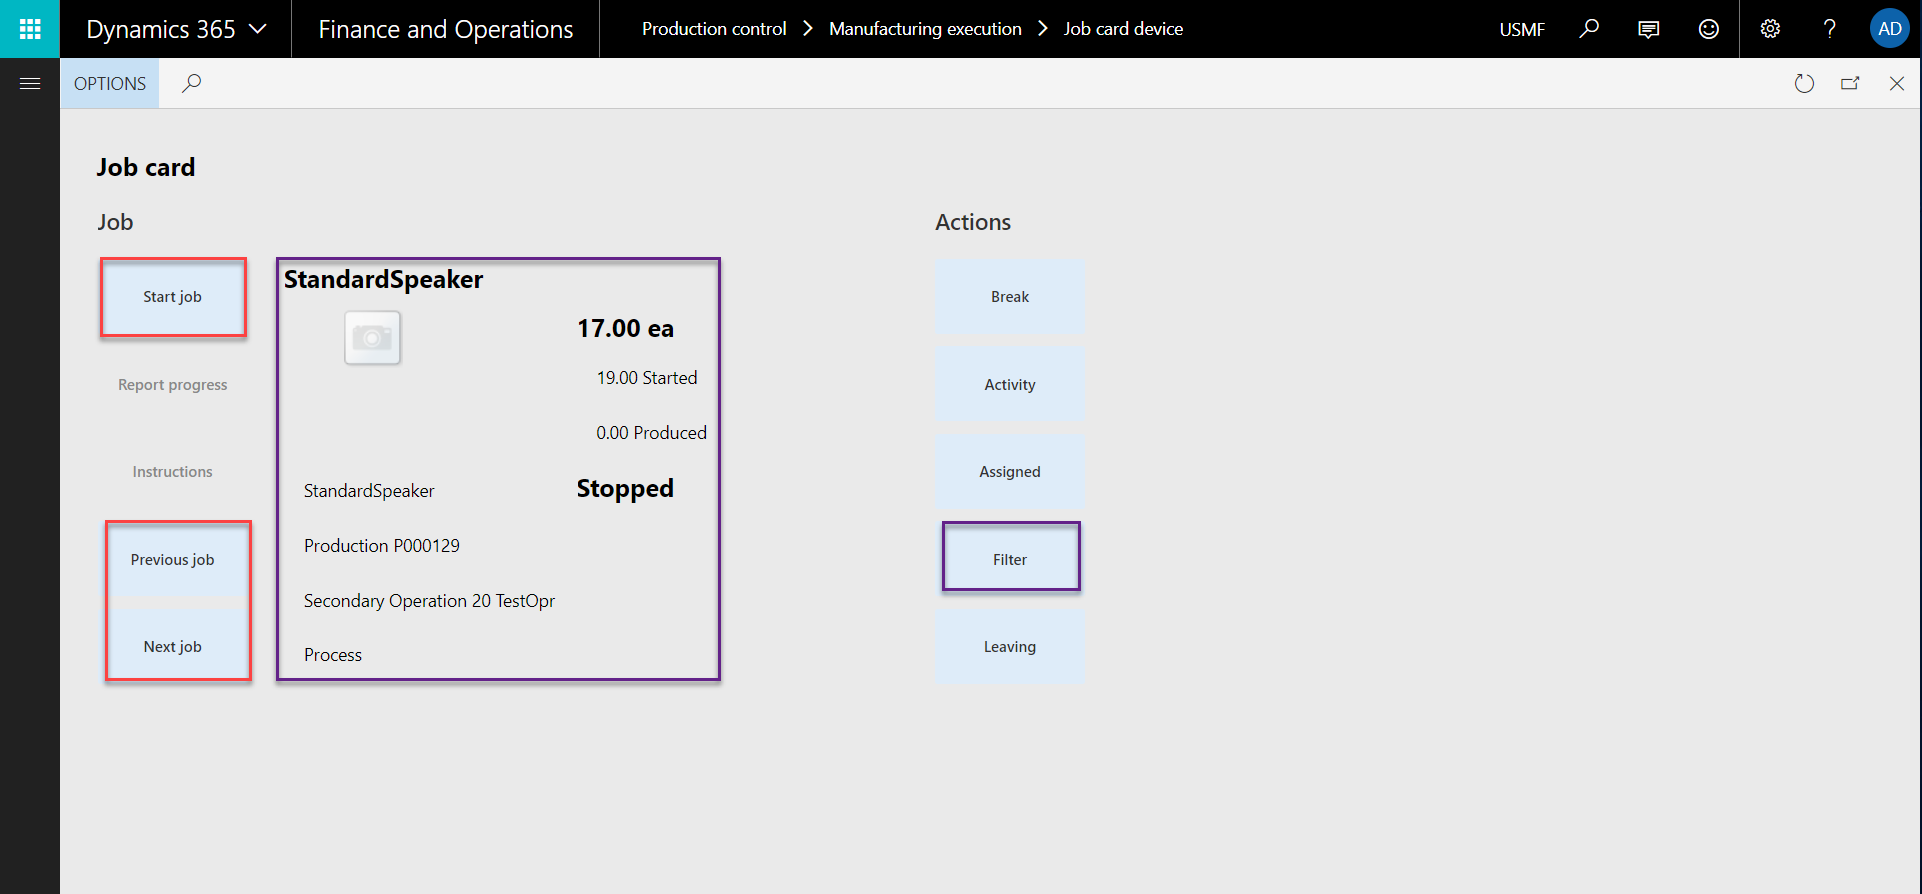
\includegraphics[width=0.8\textwidth]{img/d365productionControl4.png}
    \caption{Job Card Device module}
\end{figure}
Indeling scherm: De linkerzijde (zie rode kaders) omvat functionaliteiten die van toepassing zijn op een productie order. De knoppen aangeduid met een kader zullen in de chatbot verwerkt worden. Zo zal het dus mogelijk zijn om een job te starten (of stoppen, indien van toepassing), en om te navigeren tussen verschillende productie orders. De paarse kaders zullen ook verwerkt worden, namelijk in die zin dat het ook mogelijk zal zijn om informatie te zien over een productie order. Aanvullend zal er in de chatbot ook per productie order een bill of materials getoond worden. Dit was een extra requirement van de opdrachtgever (delaware), want een BOM is immers zeer relevante informatie voor een productiemedewerker. 


\section{Proof of concept}
Bij het onderzoek werd eerst een functionele analyse gemaakt op maat van het beoogde proof of concept. Allereerst werd hiervoor een user story opgemaakt om de scope van het onderzoek te bepalen. In onderstaande afbeelding ziet men een visuele representatie van het BPMN diagram. Voor een afbeelding op ware grootte kunnen de bijlagen geraadpleegd worden. 

\begin{figure}[h]
    \centering
    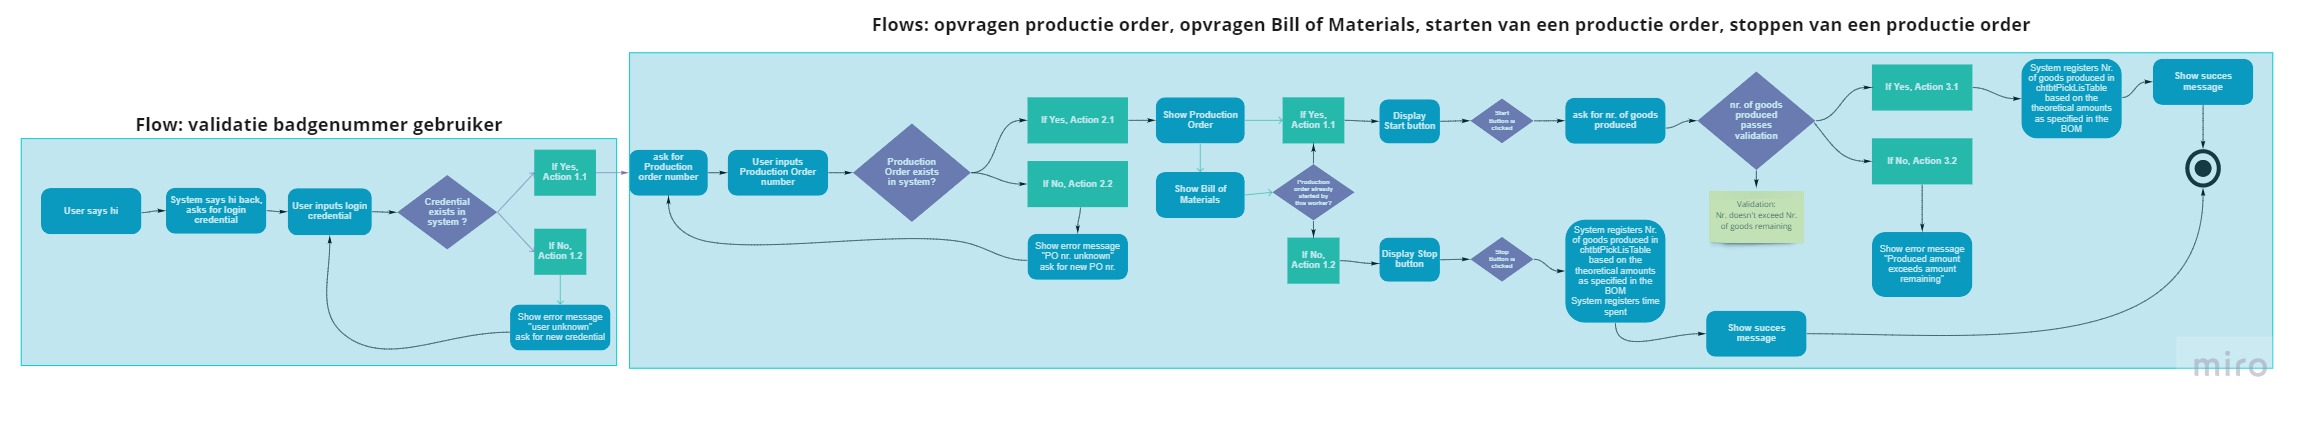
\includegraphics[width=1\textwidth]{img/HappyFlows.jpg}
    \caption{Business Process Model and Notation diagram POC }
\end{figure}

Enkele belangrijke opmerkingen: 
Het linkerdeel van het BPMN omvat must-have 5 (zie functionele requirements hieronder). Van zodra deze stap voldaan is kan de gebruiker acties uitvoeren in de chatbot, en niet eerder. Deze stap zal dus recurrent voorkomen bij alle functionaliteiten van de bot.

Verder zullen er er ook nog andere functionaliteiten in zitten die niet in het BPMN gedefinieerd zijn. Voorbeelden hiervan zijn nice to haves 3 en 4. Aangezien de flows voor deze functionaliteiten uit zéér weinig stappen bestaan, en dus in enige mate triviaal zijn. Daarom werd het opstellen van flows voor deze stappen als buiten de scope van dit onderzoek beschouwd. 

\subsubsection{functionele requirements}

Must haves:
\begin{enumerate}
    \item Er wordt een proof-of-concept gebouwd in het Microsoft Bot Framework. 
    \item Bovengenoemde bot gebruikt LUIS voor het interpreteren van natuurlijke zinnen naar commando's. 
    \item Ook moet de bot gepaste CRUD operaties kunnen uitvoeren in D365FO.
    \item De gebruiker kan inloggen adhv een badgeID (zonder deze badgeID kan de gebruiker niks doen. Validatie: badgeID bestaat in D365FO.)
    \item Eens ingelogd kan de gebruiker een aantal acties beginnen die voor hem van toepassing zijn:  
    \subitem De gebruiker kan een productieorder bekijken (titel, hoeveelheid en productieordernummer).
    \subitem De gebruiker kan de bill of materials zien van een productieorder (verschillende onderdelen, hoeveelheid en hoeveelheid per series)
    \subitem De gebruiker kan een productieorder starten. Hiervoor moet hij eerst een hoeveelheid invullen (validatie: hoeveelheid is kleiner of gelijk aan de resterende hoeveelheid)
    \subitem De gebruiker kan een productieorder stoppen (validatie: dit is enkel mogelijk als de gebruiker deze actie heeft gestart.) 
    
\end{enumerate}

Nice to haves:
\begin{enumerate}
    \item De gebruiker kan aan de hand van spraakherkenning communiceren met de bot.
    \item De gebruiker kan aan de hand van stemherkenning herkend worden door de bot, waardoor inloggen met badgeID niet langer noodzakelijk is
    \item De gebruiker kan aan de hand van een help-menu bekijken wat zijn opties zijn (welke stappen hij kan uitvoeren d.m.v. de bot)
    \item De gebruiker kan een overzicht zien van alle presentatie-mogelijkheden binnen de bot. Deze nice to have is louter voor presentatie doeleinden bestemd. Zo moet het mogelijk kunnen zijn om te raadplegen welke soorten informatie, en in welke vorm, allemaal raadpleegbaar zijn binnen de bot (foto's, video's, hyperlinks, etc.)
\end{enumerate}

Enkele belangrijke opmerkingen:
De focus voor dit onderzoek ligt niet op het coderen van zo veel mogelijk functionaliteiten, aangezien dit na de eerste keer veel repetitief werk met zich meebrengt. Het werd daarom als voldoende beschouwd door de opdrachtgever (delaware) wanneer er duidelijk vastgesteld kon worden dat er communicatie tussen D365FO en de bot mogelijk is (zie must have 3). Later in dit onderzoek zal samengevat worden wat de aangeraden stappen en best-practices hiervoor zijn.  Er zal daarom meer toegespitst worden op de werkwijze, en onder andere de voor- en nadelen. 

Tenslotte kunnen bovenstaande functionele requirements samenvattend weergegeven worden in volgende user stories: 

\begin{figure}[h]
    \centering
    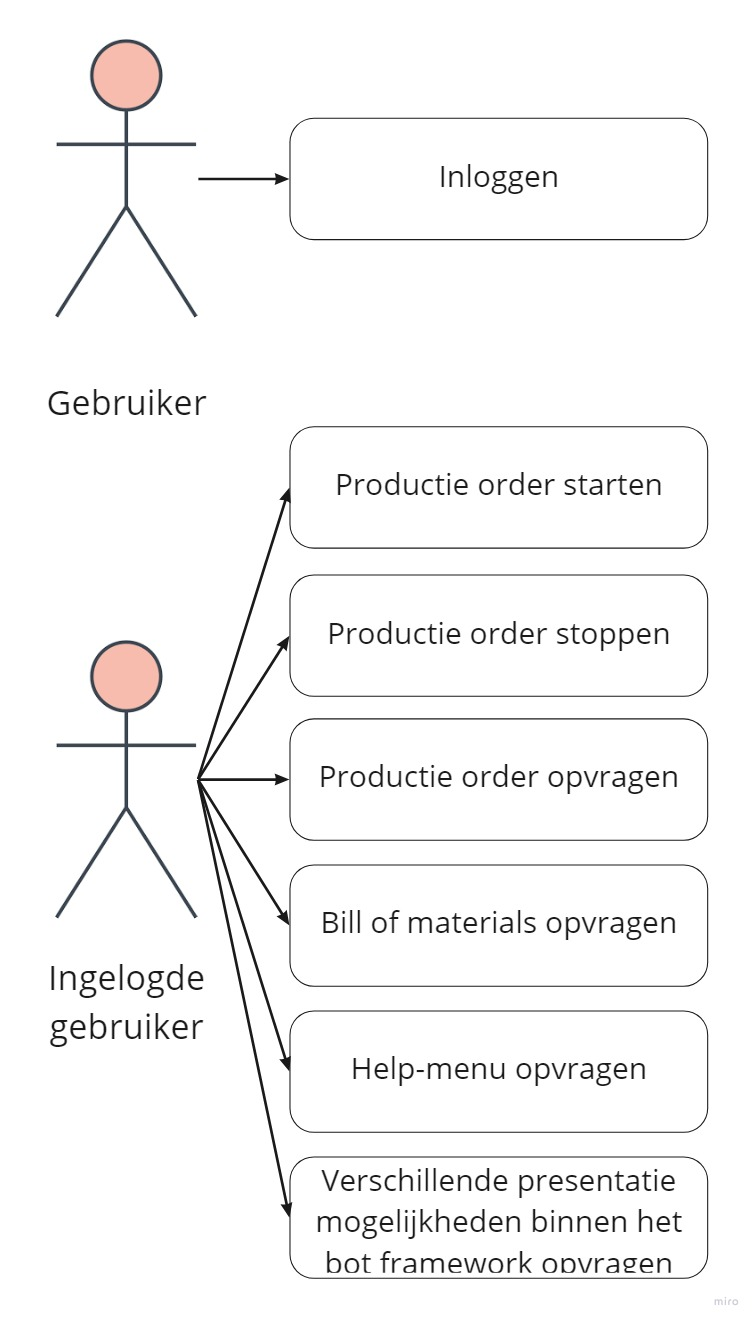
\includegraphics[width=0.32\textwidth]{img/UserStories.jpg}
    \caption{User stories POC }
\end{figure}


 

    %%%=============================================================================
%% Technische Analyse
%%=============================================================================
\chapter{Technische Analyse}
\label{ch:technischeanalyse}

\section{Architectuur}
Voor het proof of concept zullen 3 applicaties worden gemaakt:
\begin{enumerate}
    \item D365FO applicatie met eigen model ('chtbt')
    \item C\# .NET webapplicatie voor authenticatie
    \item Implementatie in het MS Bot Framework
\end{enumerate}
\begin{figure}[h]
    \centering
    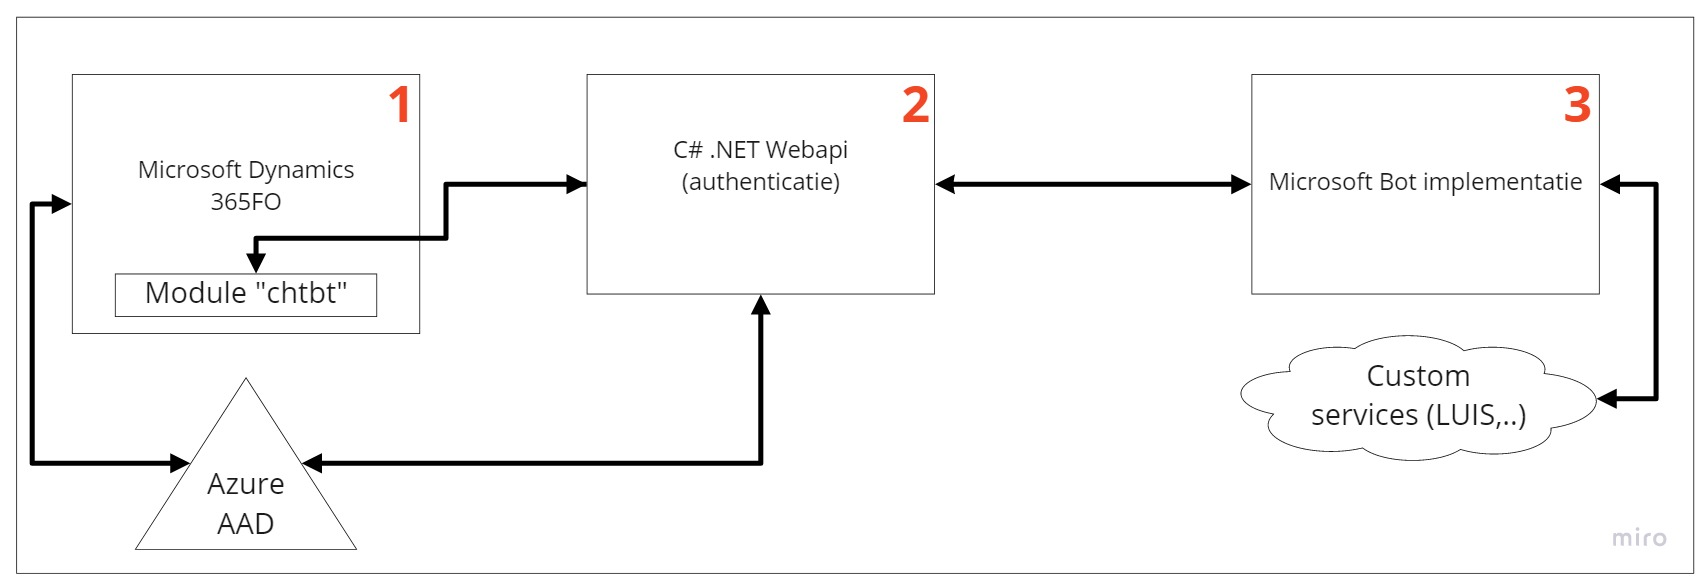
\includegraphics[width=1\textwidth]{img/ApplicatieArchitectuur}
    \caption{Applicatie architectuur}
\end{figure}
De eerste applicatie dient voor het programmeren van custom services binnen D365F0. Hiervoor zal een apart model gebouwd worden, genaamd 'chtbt' (afkorting voor chatbot). Binnen deze applicatie zal bestaande logica uit D365FO gebruikt, en beschikbaar gesteld worden d.m.v. een webservice. 

De tweede applicatie zal vervolgens connecteren met de eerste, en als communicatiemiddel dienen tussen de eerste en de derde applicatie. De reden dat hiervoor een aparte webapplicatie werd gebouwd is om de scheiding van taken en verantwoordelijkheden duidelijk af te bakenen per applicatie. Zo zal het authenticatiegedeelte (zie later) in deze omvat worden om gevoelige informatie (verbindingssleutels Azure, etc.) te verbergen voor de buitenwereld. 

Tenslotte zal uiteraard ook een chatbot gebouwd worden. Als deze dan wilt communiceren met D365FO om bepaalde CRUD-operaties uit te voeren, hoeft het enkel requests te versturen naar de authenticatie applicatie.

\section{Ontwikkel omgeving}
De ontwikkeling van het POC gebeurt volledig in de cloud, en dit op een Remote Desktop die draait op Lifecycle Services van Microsoft. Dit is een portaal waar meerdere mensen kunnen samenwerken, en dat de gebruiker assisteert in het beheren van de applicatie lifecycles van de verschillende D365FO implementaties.
Een schematische voorstelling:

\begin{figure}[H]
    \centering
    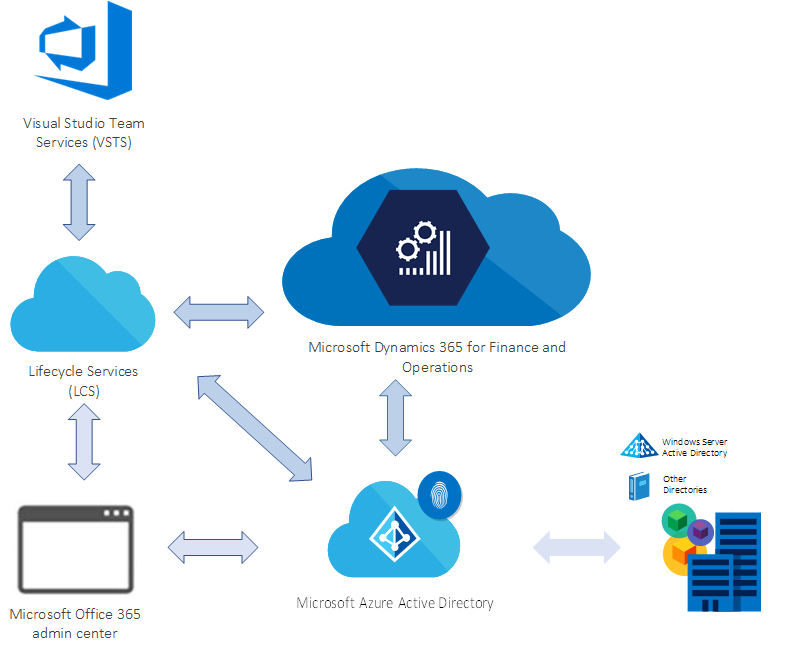
\includegraphics[width=0.8\textwidth]{img/lcsCloudArchitecture.png}
    \caption{Microsoft Lifecycle Services cloud architectuur}
\end{figure}

Aangezien dit proof of concept veel webrequests omvat, wordt er voor gekozen om deze eerst via de localhost te ontwikkelen. In een volgende stap zullen deze dan gehost worden. 

\section{Demo omgeving}
Wat betreft demo's van het poc zullen deze steeds 100\% in-cloud uitgevoerd worden. Dit wil zeggen dat alledrie de applicaties gehost zullen worden op hun respectievelijke webadressen, en de bot dus van eender waar bereikbaar, en bruikbaar is. 

De webadressen hiervoor zijn 
Insert finale webadressen
%%TODO 

\section{Authenticatie}
De authenticatie tussen Dynamics 365FO en de chatbot vereiste een aparte applicatie. Dit omdat de authenticatie volledig via Azure AAD verloopt. De authenticatie app werd geregistreerd binnen de D365FO Azure AAD applicaties (in D365FO: dashboard -> Azure Active Directory Applications). In D365FO ziet dit er als volgt uit: 
\begin{figure}[H]
    \centering
    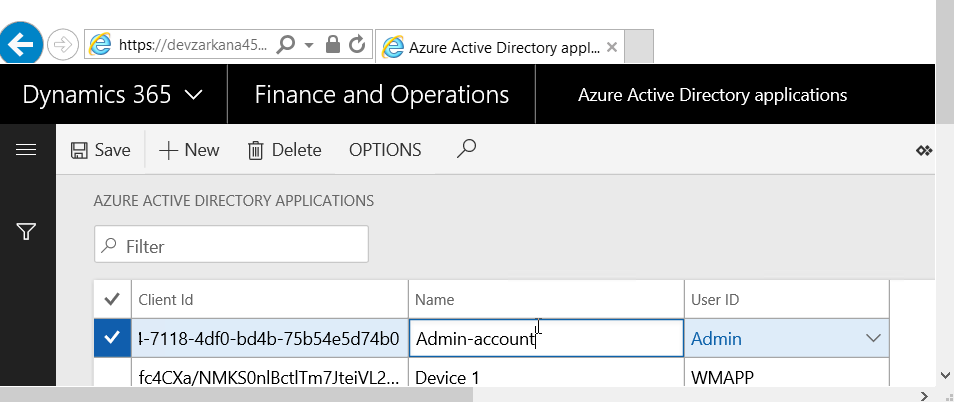
\includegraphics[width=1\textwidth]{img/impersination.png}
    \caption{Microsoft Lifecycle Services cloud architectuur}
\end{figure}
Nadat dit gebeurd is, kan er geconnecteerd worden met D365FO van buitenaf adhv. impersination. 
Dit wil zeggen dat wanneer iemand van buitenaf wilt inloggen op een d365FO omgeving, deze eerst moet inloggen op Azure om een Authorization Token te ontvangen. Vervolgens kan de gebruiker dan toegang aanvragen aan de resource (D365FO), om zo een Acces Token te kunnen bekomen. Als deze werd toegekend kan de Acces Token meegestuurd worden met alle volgende requests naar D365FO. Deze zal immers aan de Dynamics kant gevalideerd worden om dan toegang toe te kennen of te weigeren naargelang de situatie die zich voordoet. In onderstaande afbeelding wordt dit proces schematisch samengevat.

\begin{figure}[H]
    \centering
    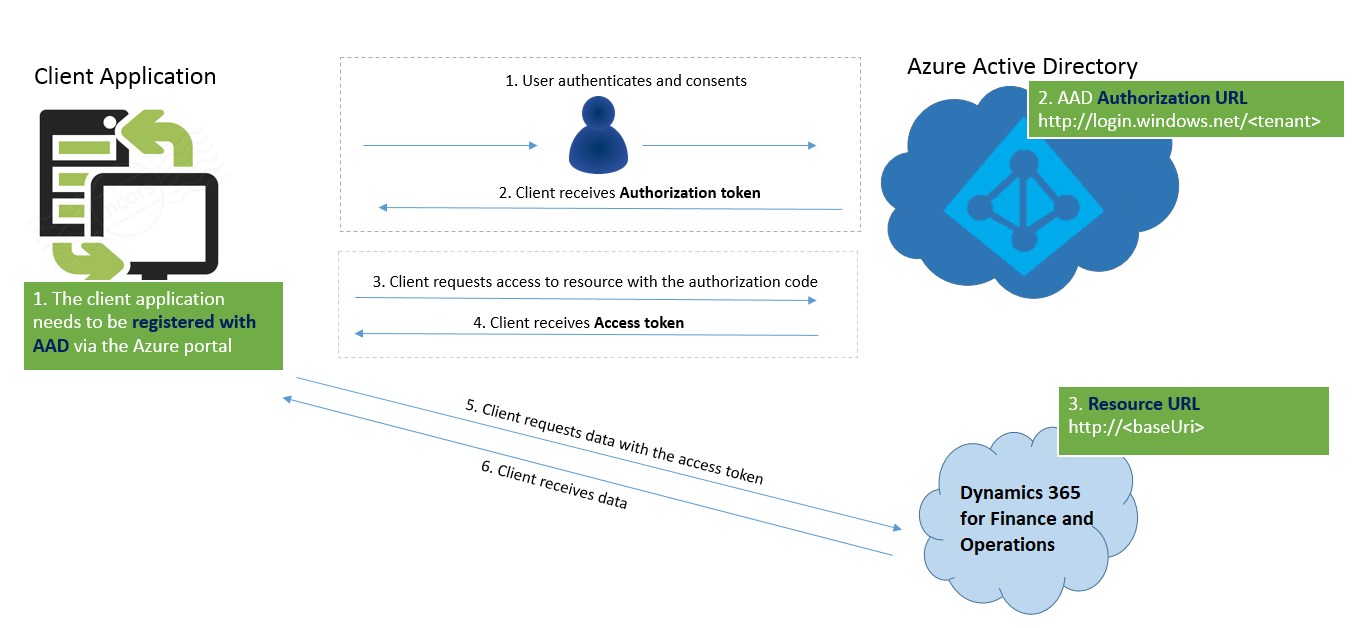
\includegraphics[width=1\textwidth]{img/aadAuthenticationArchitecture.png}
    \caption{D365FO authenticatie mbv Azure Active Directory}
\end{figure}
\subsection{Azure resources}
op het einde
\section{Data model}
Binnen D365FO zullen custom klassen en methodes gebruikt worden bovenop de reeds bestaande. De reden hiervoor is om op efficiënte manier informatie te kunnen versturen in webrequests. De bestaande klassen in D365FO zou een vorm van overkill zijn, omdat deze heel veel data bevatten die niet relevant is voor het poc. Deze klassen zullen vervolgens geserialiseerd verstuurd worden als JSON-objecten. 

\subsection{Json 2 Csharp}
De in D365FO (X++) geïmplementeerde klassen zullen vervolgens ook nodig zijn in de authenticatie app (C\#). Dit zodat de geserialiseerde JSON objecten gedeserialiseerd kunnen worden in C\# objecten. Hiervoor kan men er voor kiezen om alles dubbel te programmeren, wat dus ook dubbel werk betekent. Een andere optie is echter om de JSON strings te gebruiken voor de conversie. Hier zijn verschillende sites en tools voor, waarvan Json2Csharp.com een voorbeeld is. 
In onderstaande afbeelding wordt geïllustreerd hoe dit in zijn werk gaat. De geserialiseerde JSON string kan integraal geplakt worden, waarna de tool automatisch C\# klassen zal creëren die op hun beurt slechts gekopieerd en geplakt moeten worden in een nieuwe lege C\# klasse. 
\begin{figure}[H]
    \centering
    \includegraphics[width=1\textwidth]{img/json2Csharp.png}
    \caption{Json2Csharp voorbeeld}
\end{figure}

\section{UML}
    %\input{implementatie}
    %\input{aanbevelingen}
    
    %\input{...}
    %\input{...}
    %...
    
    %%=============================================================================
%% Conclusie
%%=============================================================================

\chapter{Conclusie}
\label{ch:conclusie}

\section{Besluit}
 De onderzoeksvraag voor dit onderzoek bestaat uit 2 deelvragen
 \begin{itemize}
     \item (a) Is het MS Bot Framework matuur genoeg om business processen binnen MS Dynamics 365FO te automatiseren? 
     \item (b) Is het implementeren van dergelijke chatbots nuttig voor D365FO? 
 \end{itemize}

Wanneer we de eerste onderzoeksvraag gaan beoordelen is het antwoord hierop positief. Er werd immers een werkende chatbot gemaakt (POC) die kon verbinden met Dynamics, en kon communiceren in 2 richtingen. Zo is er gelukt om CRUD-operaties uit te voeren vanuit de bot naar D365FO. De bot werkt met NLP, en kan dus worden beschouwd als een volwaardige chatbot. Wat wel een pijnpunt is gebleken bij dit onderzoek, is support van Microsoft zelf. In de subsectie VUL IN staat immers beschreven welke hordes zich voordeden, en in welke mate Microsoft hierin een rol speelde. 

Er moet dus een kanttekening geplaatst worden bij de woordkeuze matuur, aangezien de bot hier nog lichtjes tekortschiet. Al kan men wel gerust zijn dat Software Development Kit 4 van het MS Bot Framework, waarin deze bot werd ontwikkeld, matuur genoeg is om ingezet te worden. Alleen is het soms zoeken waarom welke fouten zich wanneer voordoen. 

Wat betreft de tweede onderzoeksvraag is het antwoord minder positief. Het implementeren van dergelijke chatbot kan nuttig zijn, maar bij MS Dynamics 365 kan de implementatie complexer zijn dan wat verwacht zou worden. Zo ligt veel van de logica in D365FO verspreid over het systeem. Dit zorgt er voor dat men al een behoorlijke kennis van Dynamics moet hebben om dit op een acceptabele termijn te kunnen realiseren. Een expert zijn in D365FO is al niet vanzelfsprekend, dus laat staan een expert D365FO met kennis van het MS Bot Framework. 


\section{Aanbevelingen}
\subsection{Voor welke systemen?}
Ideaal zou zijn dat bij het funderingssysteem (dynamics in dit onderzoek) reeds een soort van domaincontroller gedefinieerd is. Hiermee wordt bedoeld: een verzamelplaats voor alle  funtionaliteiten van een systeem(onderdeel). Dit zorgt er immers voor dat er reeds een entry point is voor binnenkomende requests vanuit de chatbot. Dan moeten deze enkel de juiste parameters voorzien indien nodig, en kunnen ze zo op dezelfde manier interageren met het systeem als voordien. 

Dynamics daarentegen gebruikt veel code die `hard-coded' in de formulieren staat. Gevolg: als men deze code elders wenst te gebruiken (buiten formulieren, bvb. voor een chatbot), dan moet al die business logica gekopieerd worden naar een andere plaats zodat de bot die kan gebruiken. Dit is redundant, en indien in een latere fase de business logica verandert, moet men hem op minimaal twee plaatsen aanpassen.

Het gebruik van chatbots, en third-party apps in het algemeen, voor optimalisaties binnen Dynamics 365FO is dus mogelijk maar de ontwikkelaar moet zeker rekening houden met een aanzienlijke overhead. 

Verder zijn alle systemen die requests van- en naar een ander systeem zoals D365FO ondersteunen te optimaliseren aan de hand van een MS Bot chatbot. 

\subsection{Voor welke toepassingen?}
Dit onderzoek werd gedaan om te bekijken of diverse en complexe data inputting taken adhv een chatbot kunnen worden geoptimaliseerd. Dit is mogelijk, maar zal niet noodzakelijk een verhoogde efficiëntie teweeg brengen. Echter zijn de mogelijkheden voor andere applicaties vrijwel onbeperkt. 

Zo is het framework heel sterk in informatieweergave (adaptive cards). Vrijwel alle soorten data kunnen op een gestructureerde manier worden weergegeven. Dit zorgt voor een grote bruikbaarheid binnen andere business cases, bijvoorbeeld bij een case waarbij productiemedewerkers complexe stappen (evt. op maat) moeten doorlopen om een goed te produceren. Zo kunnen ze steeds op een snelle en handige manier nodige info raaplegen vanuit het systeem. 

Ook mag men niet verwaarlozen hoe sterk de NLP-engine LUIS is. Deze is zeer sterk in het snel interpreteren van natuurlijke tekst, en dankzij de geïntegreerde machine learning zal het model enkel verbeteren in functie van de tijd. Zo kan een chatbot gebouwd worden als een soort van meta-applicatie. Stel bijvoorbeeld dat een bedrijf interne softwaremodules heeft voor zijn medewerkers. Bijvoorbeeld een voor het ingeven van hun onkosten, een voor het inchekken, een voor afwezigheid te melden, enzovoort. Een bot van het MS Bot framework kan dan perfect dienen als een soort van meta-applicatie. De gebruiker zegr wat hij wil doen, en de bot stuurt de gebruiker juist door. Dan kan er nog overwogen worden om voor die afzonderlijke apps formulieren aan te maken in de bot zelf om de integratie zo volledig te doen. Ook kan er doorverwezen worden naar de juiste applicatie. Heel veel mogelijkheden dus. 





% TODO: Trek een duidelijke conclusie, in de vorm van een antwoord op de
% onderzoeksvra(a)g(en). Wat was jouw bijdrage aan het onderzoeksdomein en
% hoe biedt dit meerwaarde aan het vakgebied/doelgroep? 
% Reflecteer kritisch over het resultaat. In Engelse teksten wordt deze sectie
% ``Discussion'' genoemd. Had je deze uitkomst verwacht? Zijn er zaken die nog
% niet duidelijk zijn?
% Heeft het onderzoek geleid tot nieuwe vragen die uitnodigen tot verder 
%onderzoek?



    
    %%=============================================================================
    %% Bijlagen
    %%=============================================================================
    
    \appendix
    \renewcommand{\chaptername}{Appendix}
    
    %%---------- Onderzoeksvoorstel -----------------------------------------------
    
    \chapter{Onderzoeksvoorstel}
    
    Het onderwerp van deze bachelorproef is gebaseerd op een onderzoeksvoorstel dat vooraf werd beoordeeld door de promotor. Dat voorstel is opgenomen in deze bijlage.
    
    % Verwijzing naar het bestand met de inhoud van het onderzoeksvoorstel
    %---------- Inleiding ---------------------------------------------------------

\section{Introductie} % The \section*{} command stops section numbering
\label{sec:introductie}
Delaware is een vooruitstrevende organisatie. Dit wil zeggen dat men steeds bezig is met het onderzoeken en ontwikkelen van "next-functionality"  zodat ze klaar zijn om in productie te gaan van zodra de markten hier rijp voor zijn. Echter blijft de Data-inputting voor vele organisaties een lastig onderdeel dat veel tijd en middelen in beslag neemt. Het gebruiken van Cognitive services en bots klinkt hiervoor zeer veelbelovend, maar zal het gebruik hiervan ook binnen een professionele ERP-omgeving nog kunnen zorgen voor toegevoegde waarde? Dit zal onderzocht worden enerzijds, maar anderzijds zal er ook een proof of concept gemaakt worden binnen Microsoft Dynamics ERP. 


%---------- Stand van zaken ---------------------------------------------------

\section{State-of-the-art}
\label{sec:state-of-the-art}
Er zijn reeds gelijkaardige onderzoeken gevoerd naar de integratie van cognitive services in ERP. Zo is er~\autocite{RizkyDharana2017}, de conclusie hiervan was dat de integratie tussen chatbots en ERP-systemen managers zullen helpen om effectiever en efficiënter te voldoen aan klantbehoeften. Echter werd hier geen onderzoek naar de rendabiliteit van genoemde integraties. In een ander werk ~\autocite{Baat2016} concludeerde men de mix tussen mensen - processen - technologie drastisch zal veranderen omwille van AI. Zo zullen veel (data-inputting) taken die tot op vandaag door mensen worden verricht, geautomatiseerd kunnen worden. Omdat een winstgevende organisatie, zoals Delaware, steeds als doelstelling heeft om operationele kosten te minimaliseren, is het daarom belangrijk dat dit onderzoek gevoerd wordt naar de rendabiliteit van de integratie tussen ERP en Cognitive services \& AI. 
% Voor literatuurverwijzingen zijn er twee belangrijke commando's:
% \autocite{KEY} => (Auteur, jaartal) Gebruik dit als de naam van de auteur
%   geen onderdeel is van de zin.
% \textcite{KEY} => Auteur (jaartal)  Gebruik dit als de auteursnaam wel een
%   functie heeft in de zin (bv. ``Uit onderzoek door Doll & Hill (1954) bleek
%   ...'')
%---------- Methodologie ------------------------------------------------------
\section{Methodologie}
\label{sec:methodologie}

Dit onderzoek zal verricht worden door de productie van een proof of concept waarin verschillende cognitive services gekoppeld aan AI getest zullen worden in een integratie met Microsoft Dynamics ERP. Dit zal in eerste instantie een chatbot zijn, en kan later uitgebreid worden. 

%---------- Verwachte resultaten ----------------------------------------------
\section{Verwachte resultaten}
\label{sec:verwachte_resultaten}

Ik verwacht dat de integratie met ERP zal lukken, aangezien hier al voorbeelden van zijn.  Daarentegen verwacht ik niet dat de technologie al klaar is om heel complexe en dynamische data-inputting taken te automatiseren. Echter moet het volgens mij wel mogelijk zijn om (relatief) simpele intents te herkennen en verwerken.  

%---------- Verwachte conclusies ----------------------------------------------
\section{Verwachte conclusies}
\label{sec:verwachte_conclusies}

De onderzoeksvraag is in dit geval zeer tijdsgebonden. Het is geen vraag meer of cognitive services, gekoppeld aan AI, een meerwaarde zullen bieden aan B2B softwaresystemen, met name ERP. Echter ben ik er niet van overtuigd dat de technologie hier al klaar voor is. Daarom denk ik dat er nog te veel bedrijfseigen aanpassingen zullen moeten gebeuren per business case waarop deze services worden toegepast, en daarom moeilijk rendabel zullen zijn. 


    
    %%---------- Andere bijlagen --------------------------------------------------
    % TODO: Voeg hier eventuele andere bijlagen toe
    %\input{...}
    
    %%---------- Referentielijst --------------------------------------------------
    
    \printbibliography[heading=bibintoc]
    
\end{document}}